\section{Experimental Evaluation}
%TODO

\subsection{Methodologies}
%Detalhes de forma a que se alguem quiser replicar os testes, consiga:
%Tipo de hardware(caractristicas)
%Parametros dos protocolos
%Run execution (tempo de execucao)
%Processamento especial às medidas?
Nesta avaliação utilizamos o Cluster do Departamento de Informática da Faculdade de Ciências e Tecnologias da Universidade Nova de Lisboa \cite{cluster}. Neste Cluster foram utilizados 2 nós (nós 5 e 6) cujo as suas características podem ser analisadas no anexo 1. Tal como referido nas secções anteriores, foram implementados quatro algoritmos, sendo dois de \textit{Partial Membership} e outros dois de \textit{Gossip Dissemination}. Como tal, foram feitos quatro testes, que combinados, geram todas as combinações dos algoritmos a funcionarem uns com os outros. As combinações foram as seguintes:
\begin{itemize}
    \item Eager Push + HyParView
    \item Eager Push + Cyclon
    \item Plumtree + HyParView
    \item Plumtree + Cyclon
\end{itemize}

Para todas as combinações as configurações são iguais, assim como a quantidade nós na rede. A quantidade escolhida foi de 100 nodes. As configurações fixas e todos os testes foram as mesmas utilizadas em \cite{hyparview} \cite{plumtree}, com: 
\begin{itemize}
    \item Tamanho máximo da Active View = 5
    \item Tamanho máximo da Passive View = 30
    \item Shuffle Timer com 15 segundos de intervalo
    \item Join Timer com 1 segundo de espera
    \item k=6 
    \item c=1
    \item ARWL=6
    \item PRWL=3
    \item ka=3
    \item kp=4
\end{itemize}

Porém, variámos para cada teste de combinação de algoritmos, o tamanho do payload, tendo feito um teste com payload grande (10000 bytes) e outro pequeno (10 bytes). Também variámos a taxa de transmissão, utilizando uma taxa grande de 3 segundo e outra mais pequena de 1 segundo. Com todas estas variações de algoritmos e propriedades, chegamos a um total de 16 testes, considerando todas as suas possíveis junções.

Para além de tudo isto, ainda adicionamos testes isolados aos algoritmos de \textit{Partial Membership} de acordo com as características anteriores e configurações variáveis de payload e taxa de transmissão, o que nos adiciona aos anteriores 16 testes, mais 8, dando um total de 24 testes que iremos demonstrar nas subsecções seguintes.

\subsection{Results}
%-->resultados (gráficos melhor que tabelas)
%gráfico único com várias linhas

%TODO: Resumo geral + Plumtree erro justificação / implementacao

%--------------------------------------
Nesta secção iremos falar mais detalhadamente, sobre os resultados obtidos na experimentação dos algoritmos no Cluster do DI.

Como dito na secção anterior, os 16 testes estão divididos por combinações de protocolos, por exemplo do tipo E + C, onde o protocolo é também identificado pela sua letra inicial. Os testes efectuados aos protocolos foram de \textit{reliability}, \textit{latency}, \textit{total sent messages}, e \textit{total failed messages} em cada nó. 

Em cada gráfico é possível também observar que a cada cor correspondem as parametrizações de payload e bit rate usados.

Como se verifica nos resultados adiantes, devido a um erro durante a implementação do Plumtree, os resultados usando este algoritmo não foram os esperados.


\subsubsection{Reliability}

%TODO: Falar dos resultados
Os resultados obtidos sobre a confiabilidade das mensagens envidas na aplicação foram bastante bons e com resultados na ordem dos 100\%, excepto com a junção do Plumtree com o Cyclon, onde, na maioria dos nós na rede, se verifica uma discrepância fora do comum.

\begin{figure}
  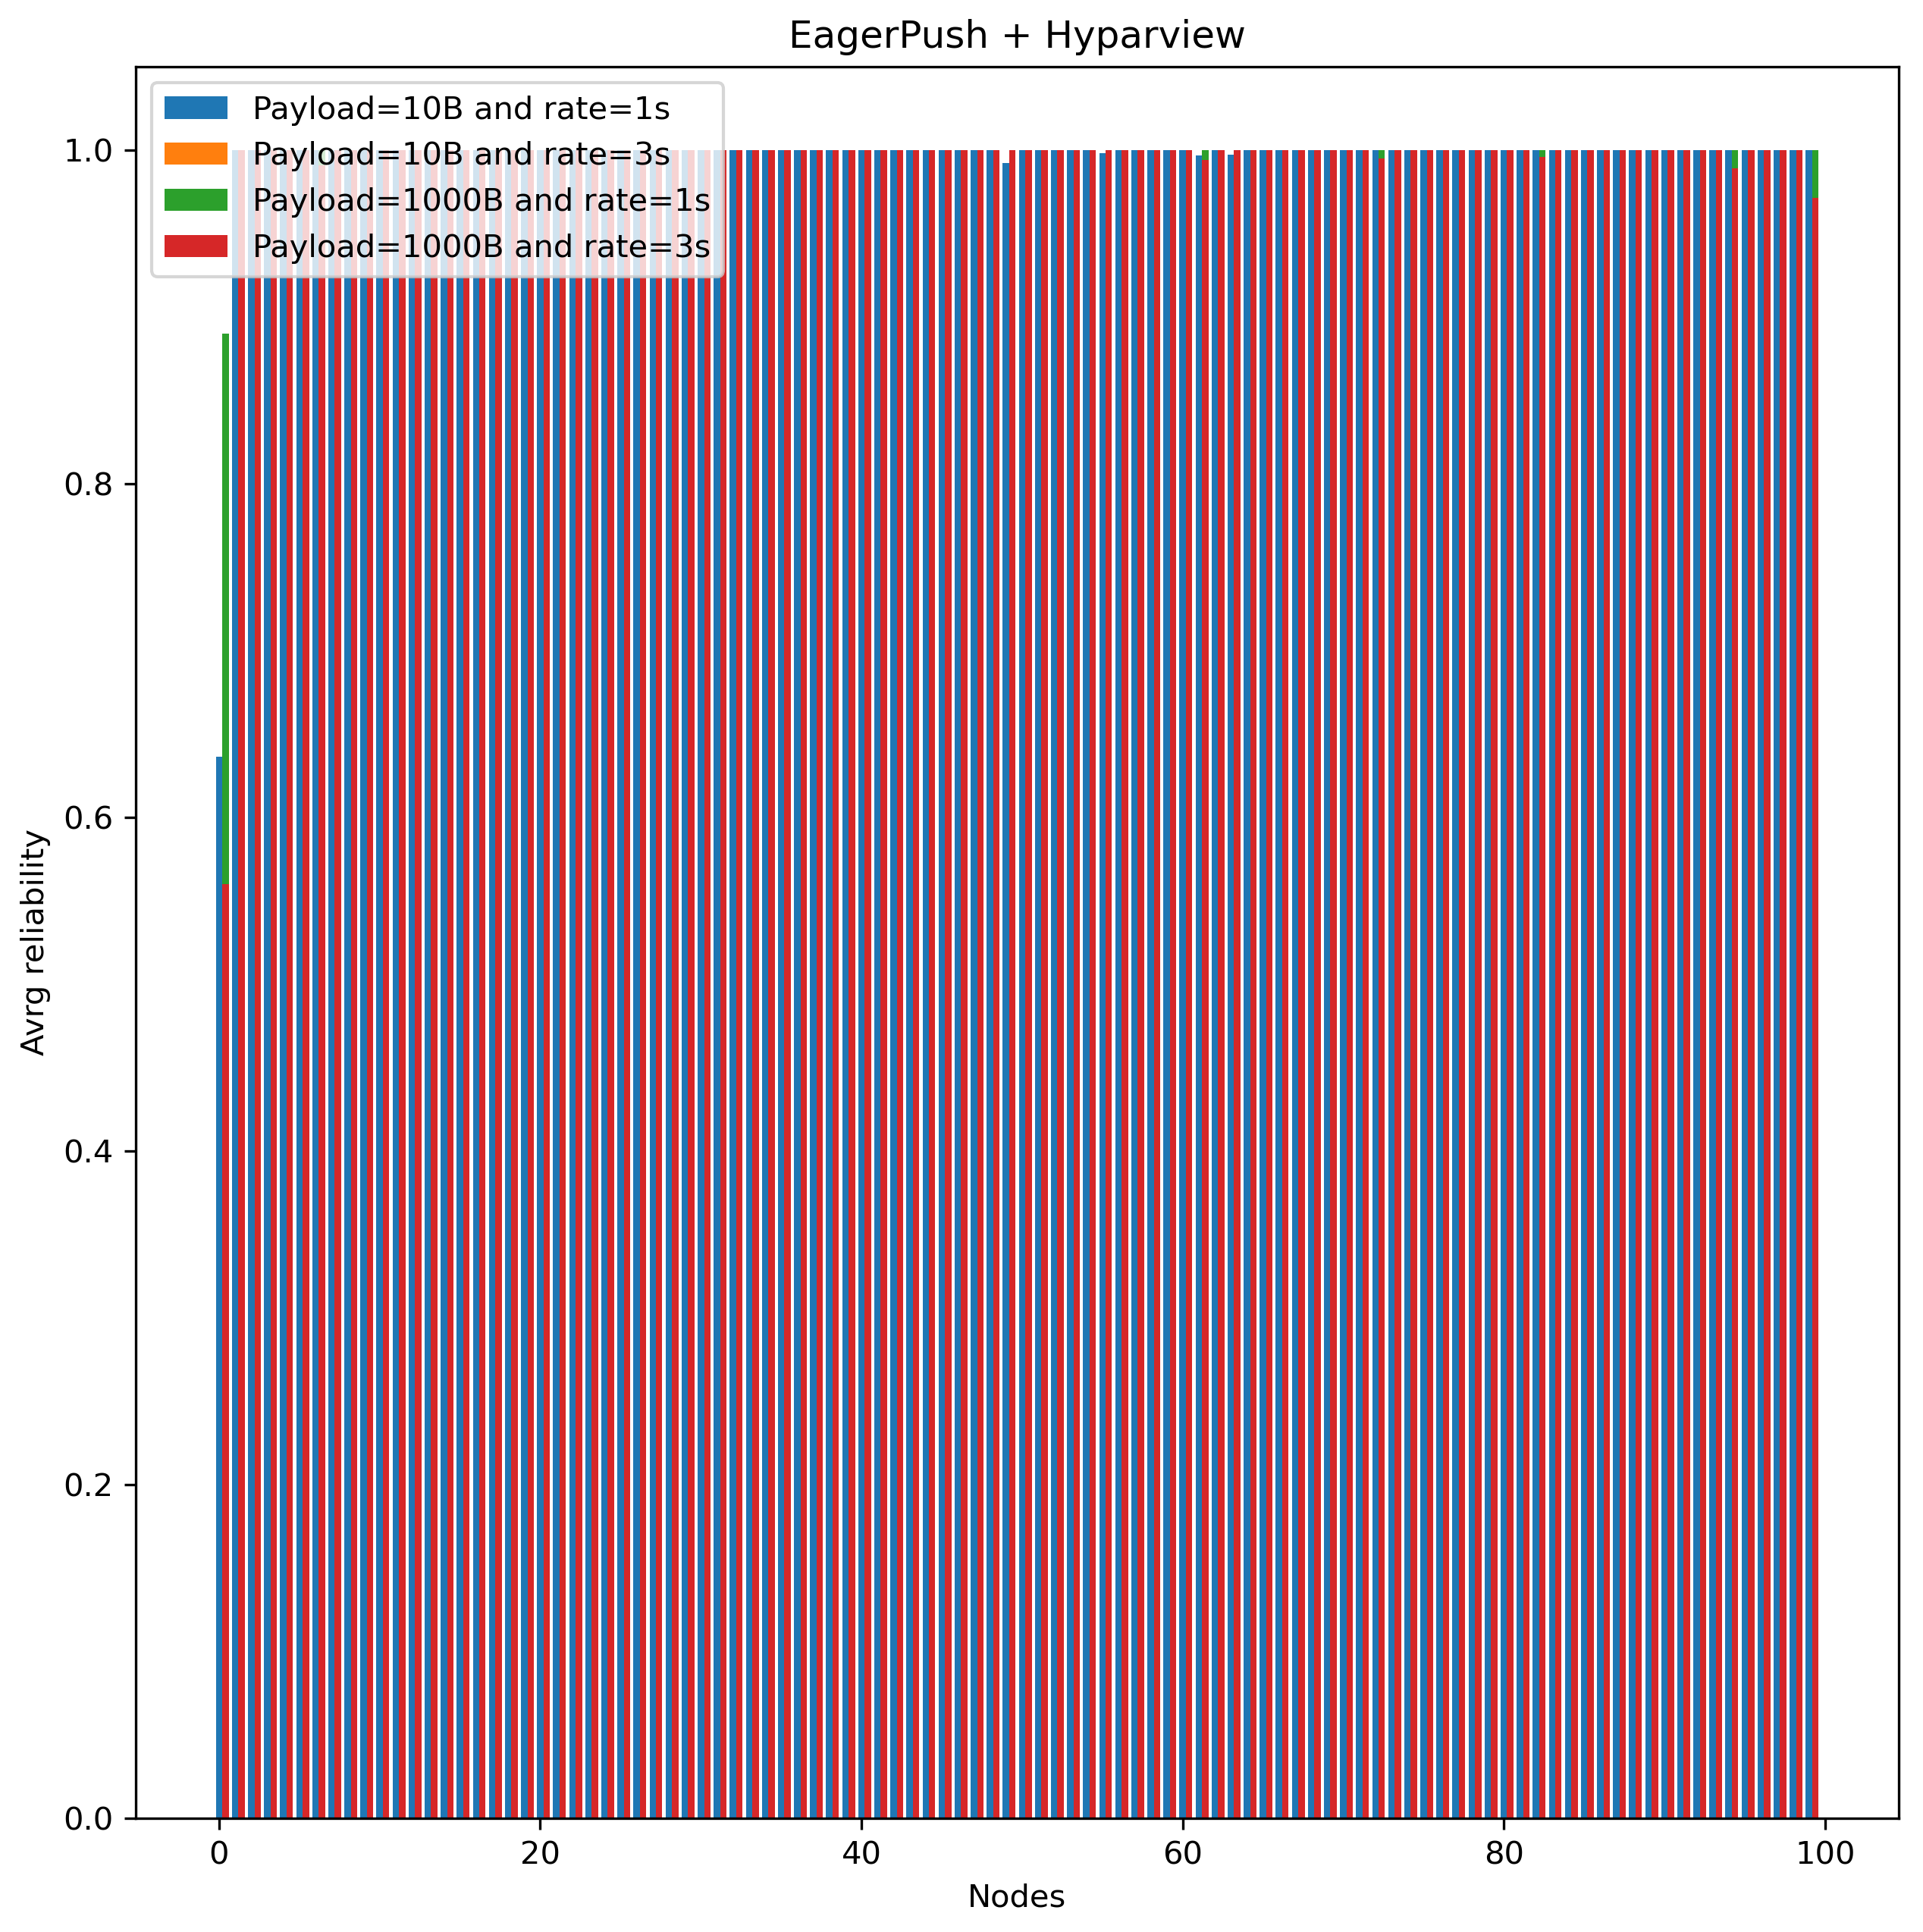
\includegraphics[width=0.4\textwidth]{images/EagerPush + HyparviewAvrg_Reliability.png}
  \caption{EagerPush + Hyparview (Reliability)}
\end{figure}

\begin{figure}
  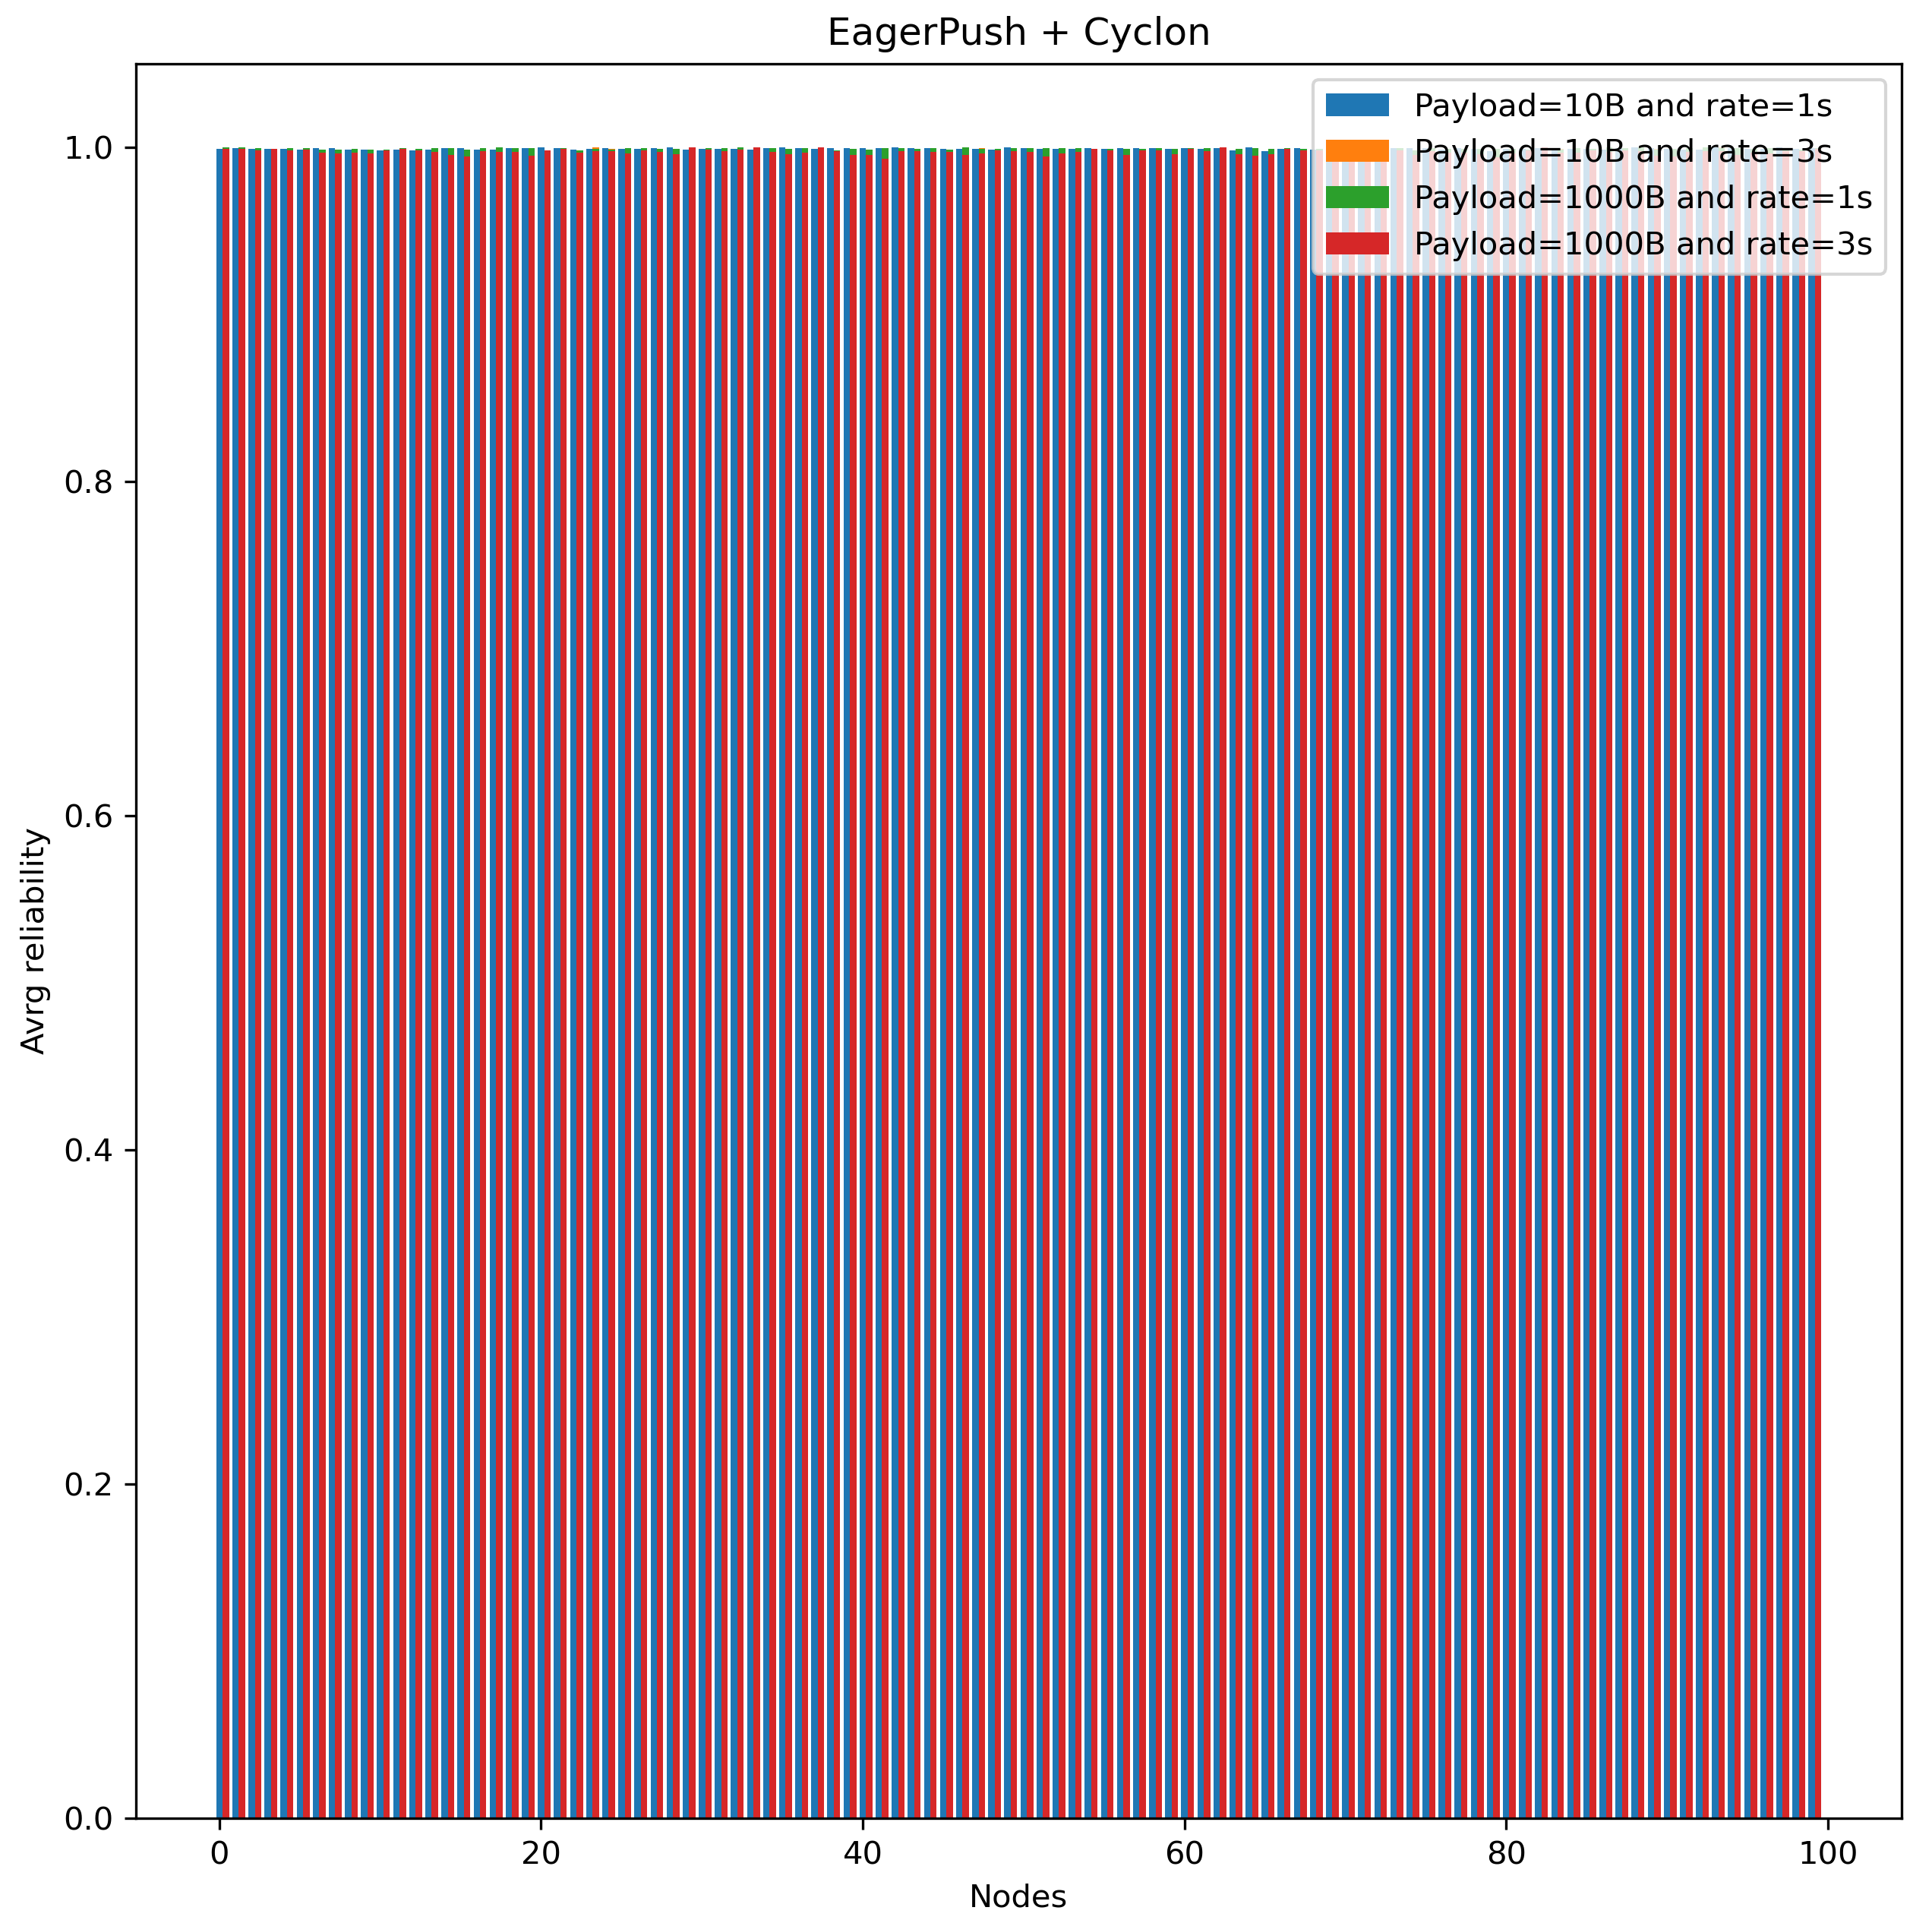
\includegraphics[width=0.4\textwidth]{images/EagerPush + CyclonAvrg_Reliability.png}
  \caption{EagerPush + Cyclon (Reliability)}
\end{figure}

\begin{figure}
  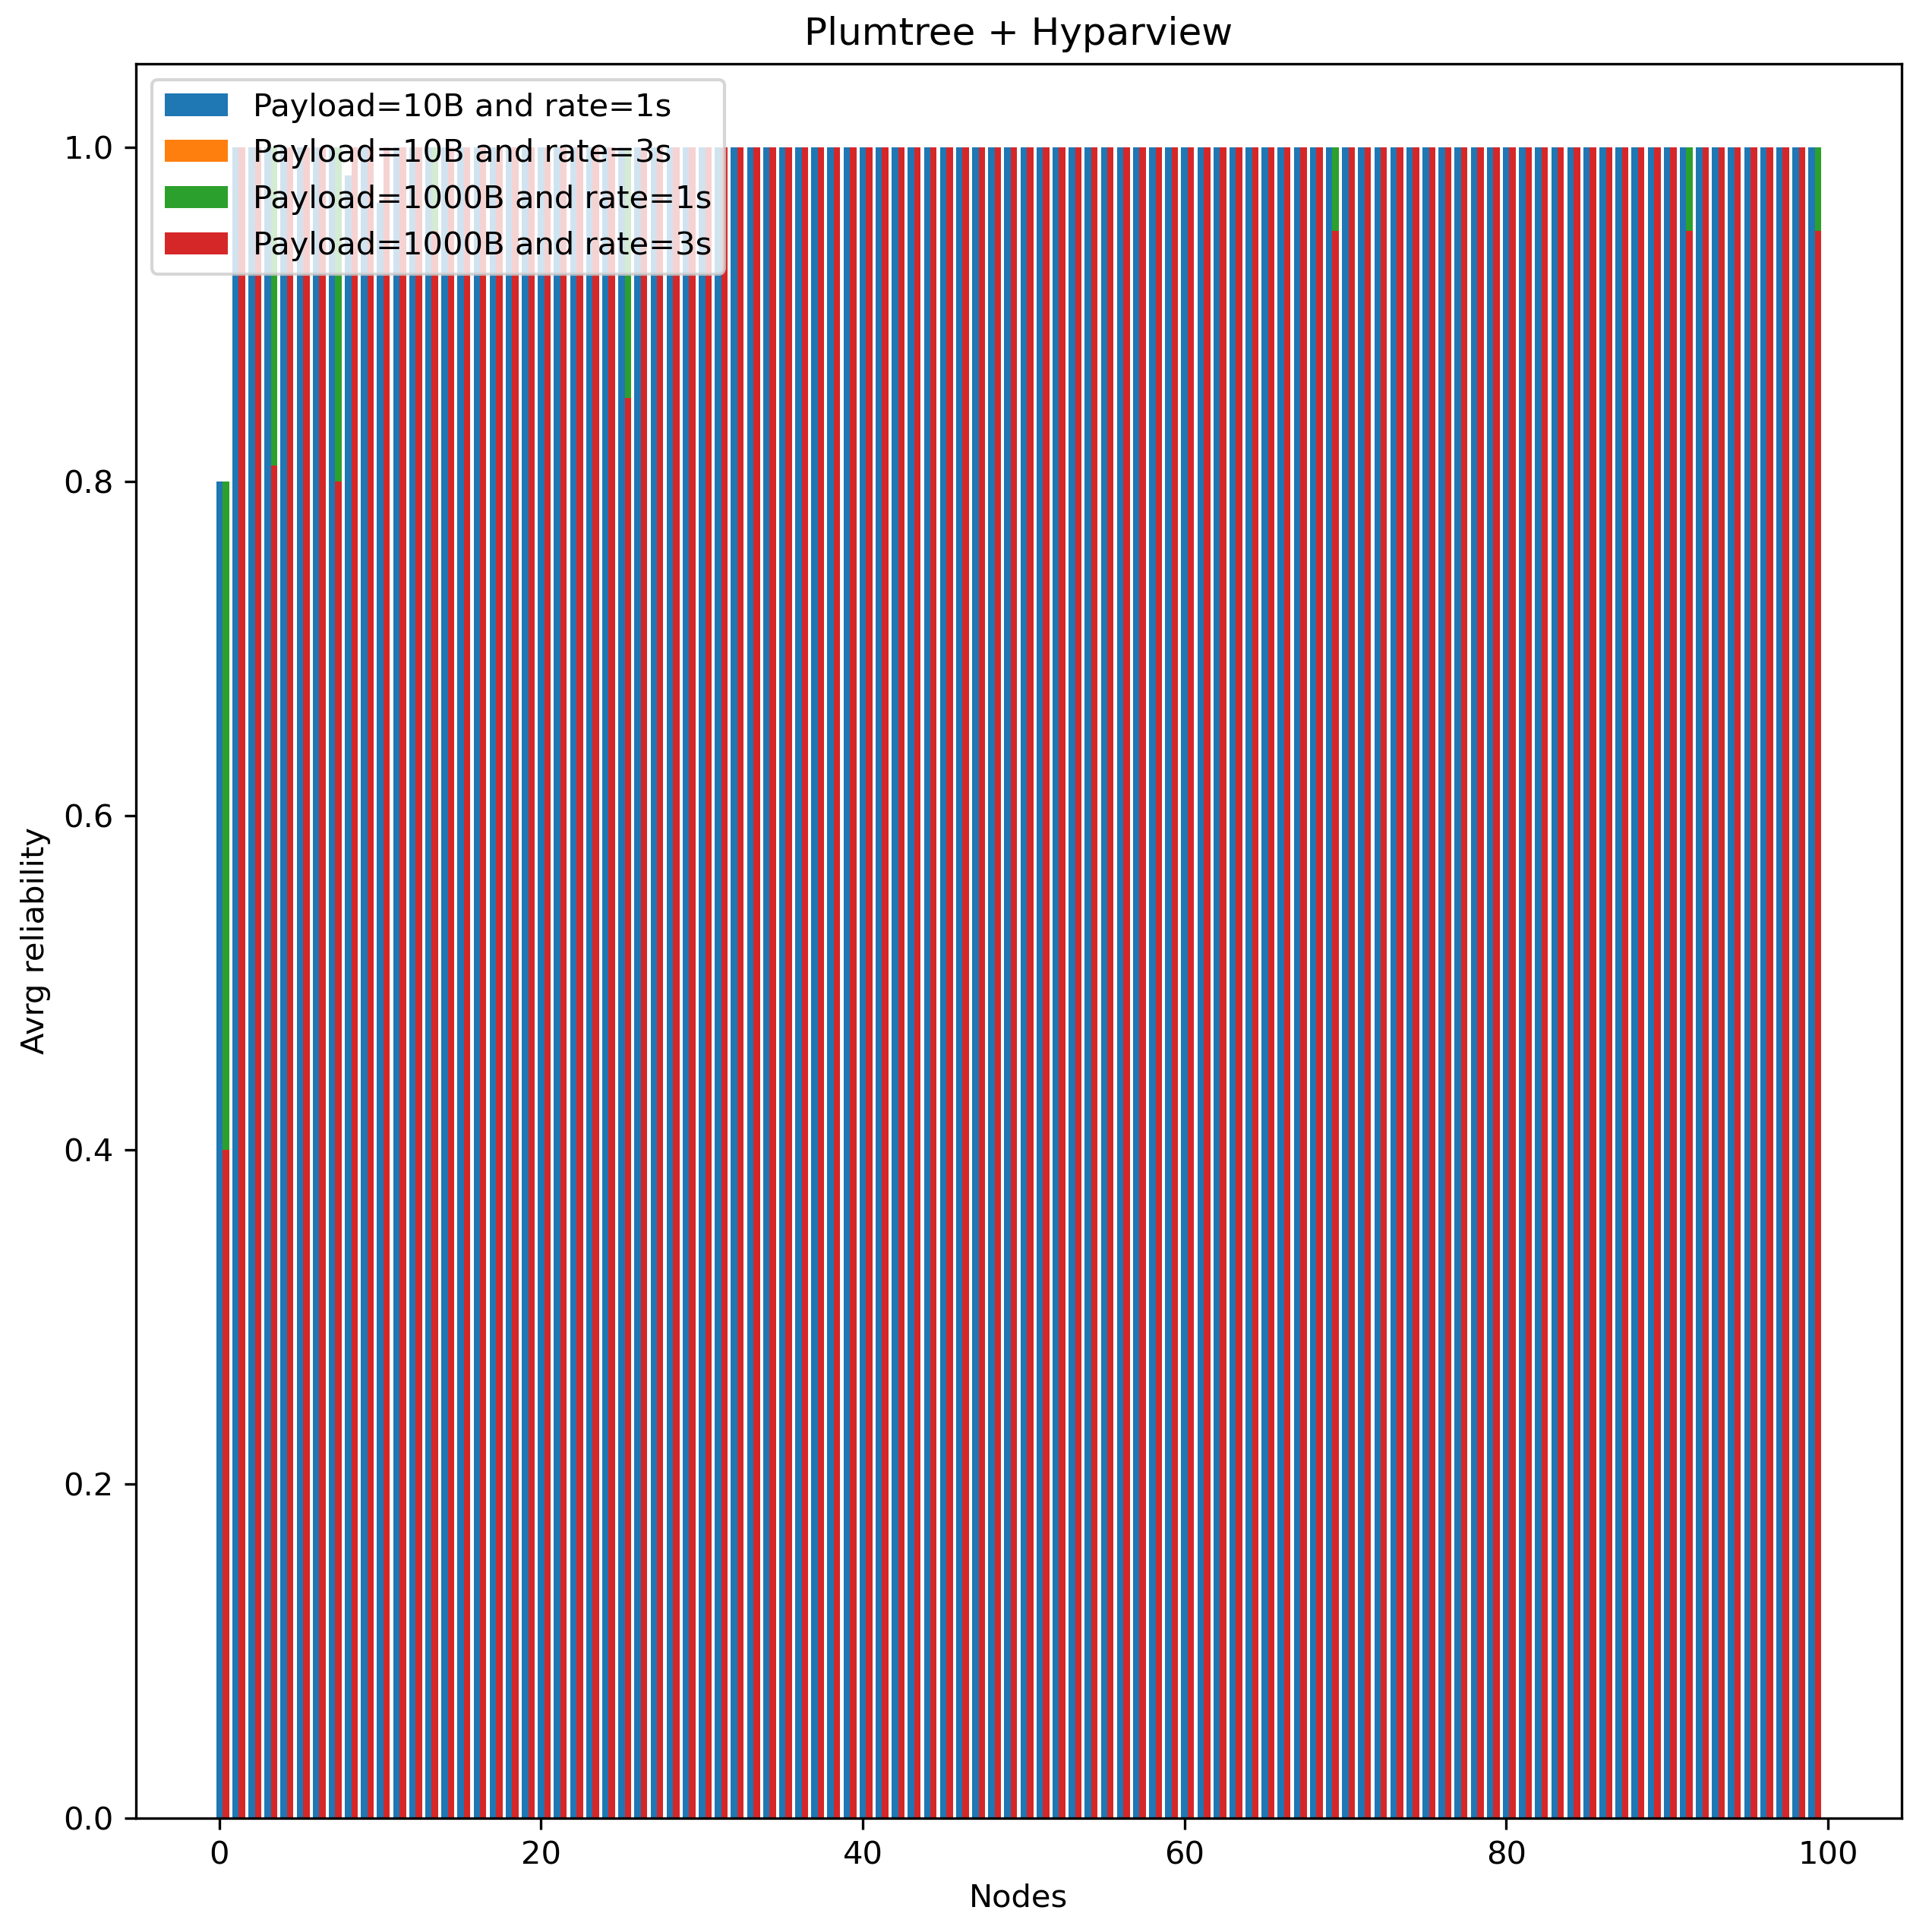
\includegraphics[width=0.4\textwidth]{images/Plumtree + HyparviewAvrg_Reliability.png}
  \caption{Plumtree + Hyparview (Reliability)}
\end{figure}

\begin{figure}
  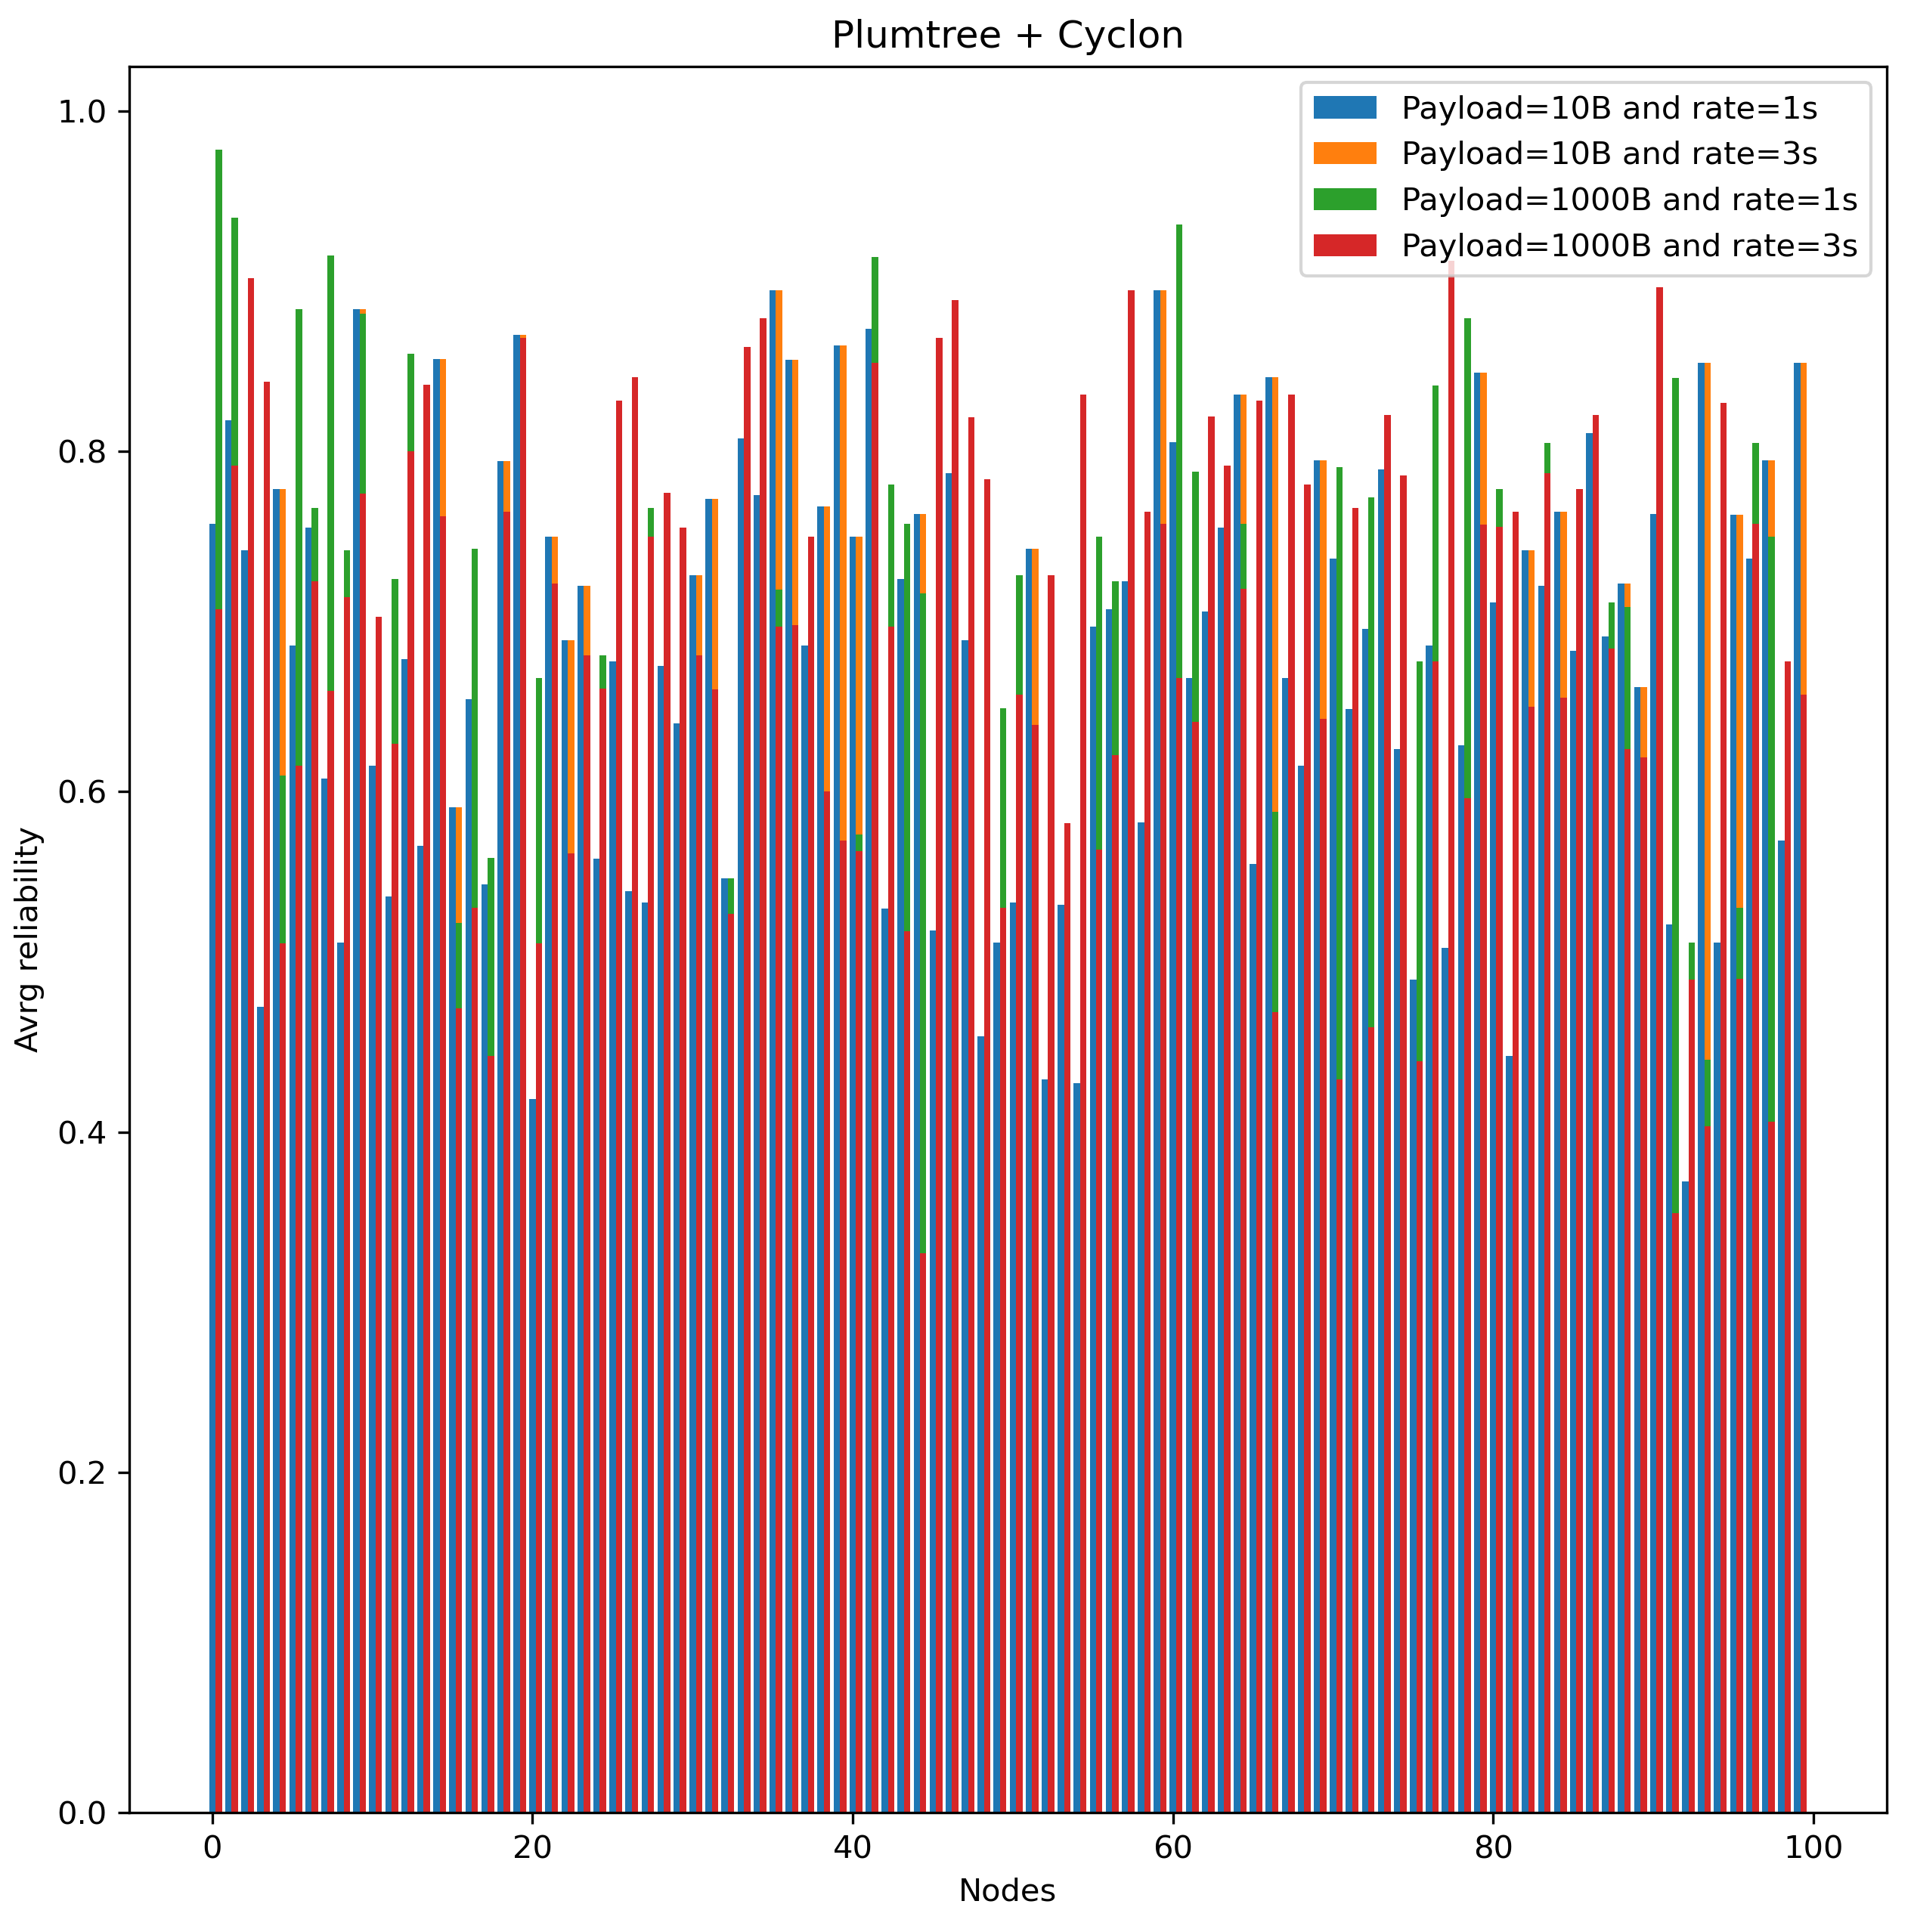
\includegraphics[width=0.4\textwidth]{images/Plumtree + CyclonAvrg_Reliability.png}
  \caption{Plumtree + Cyclon (Reliability)}
\end{figure}

%--------------------------------------

\subsubsection{Sent Messages}
Nos gráficos relativos ao envio de mensagens observa-se que na sua maioria os protocolos têm tendência a enviar menos mensagens quando o \textit{payload} destas aumenta, no entanto o Plumtree destaca-se não mostrando uma grande diferença com a alteração deste parâmetro, algo que será discutido em maior detalhe mais à frente.

%TODO: Falar dos resultados

\begin{figure}
  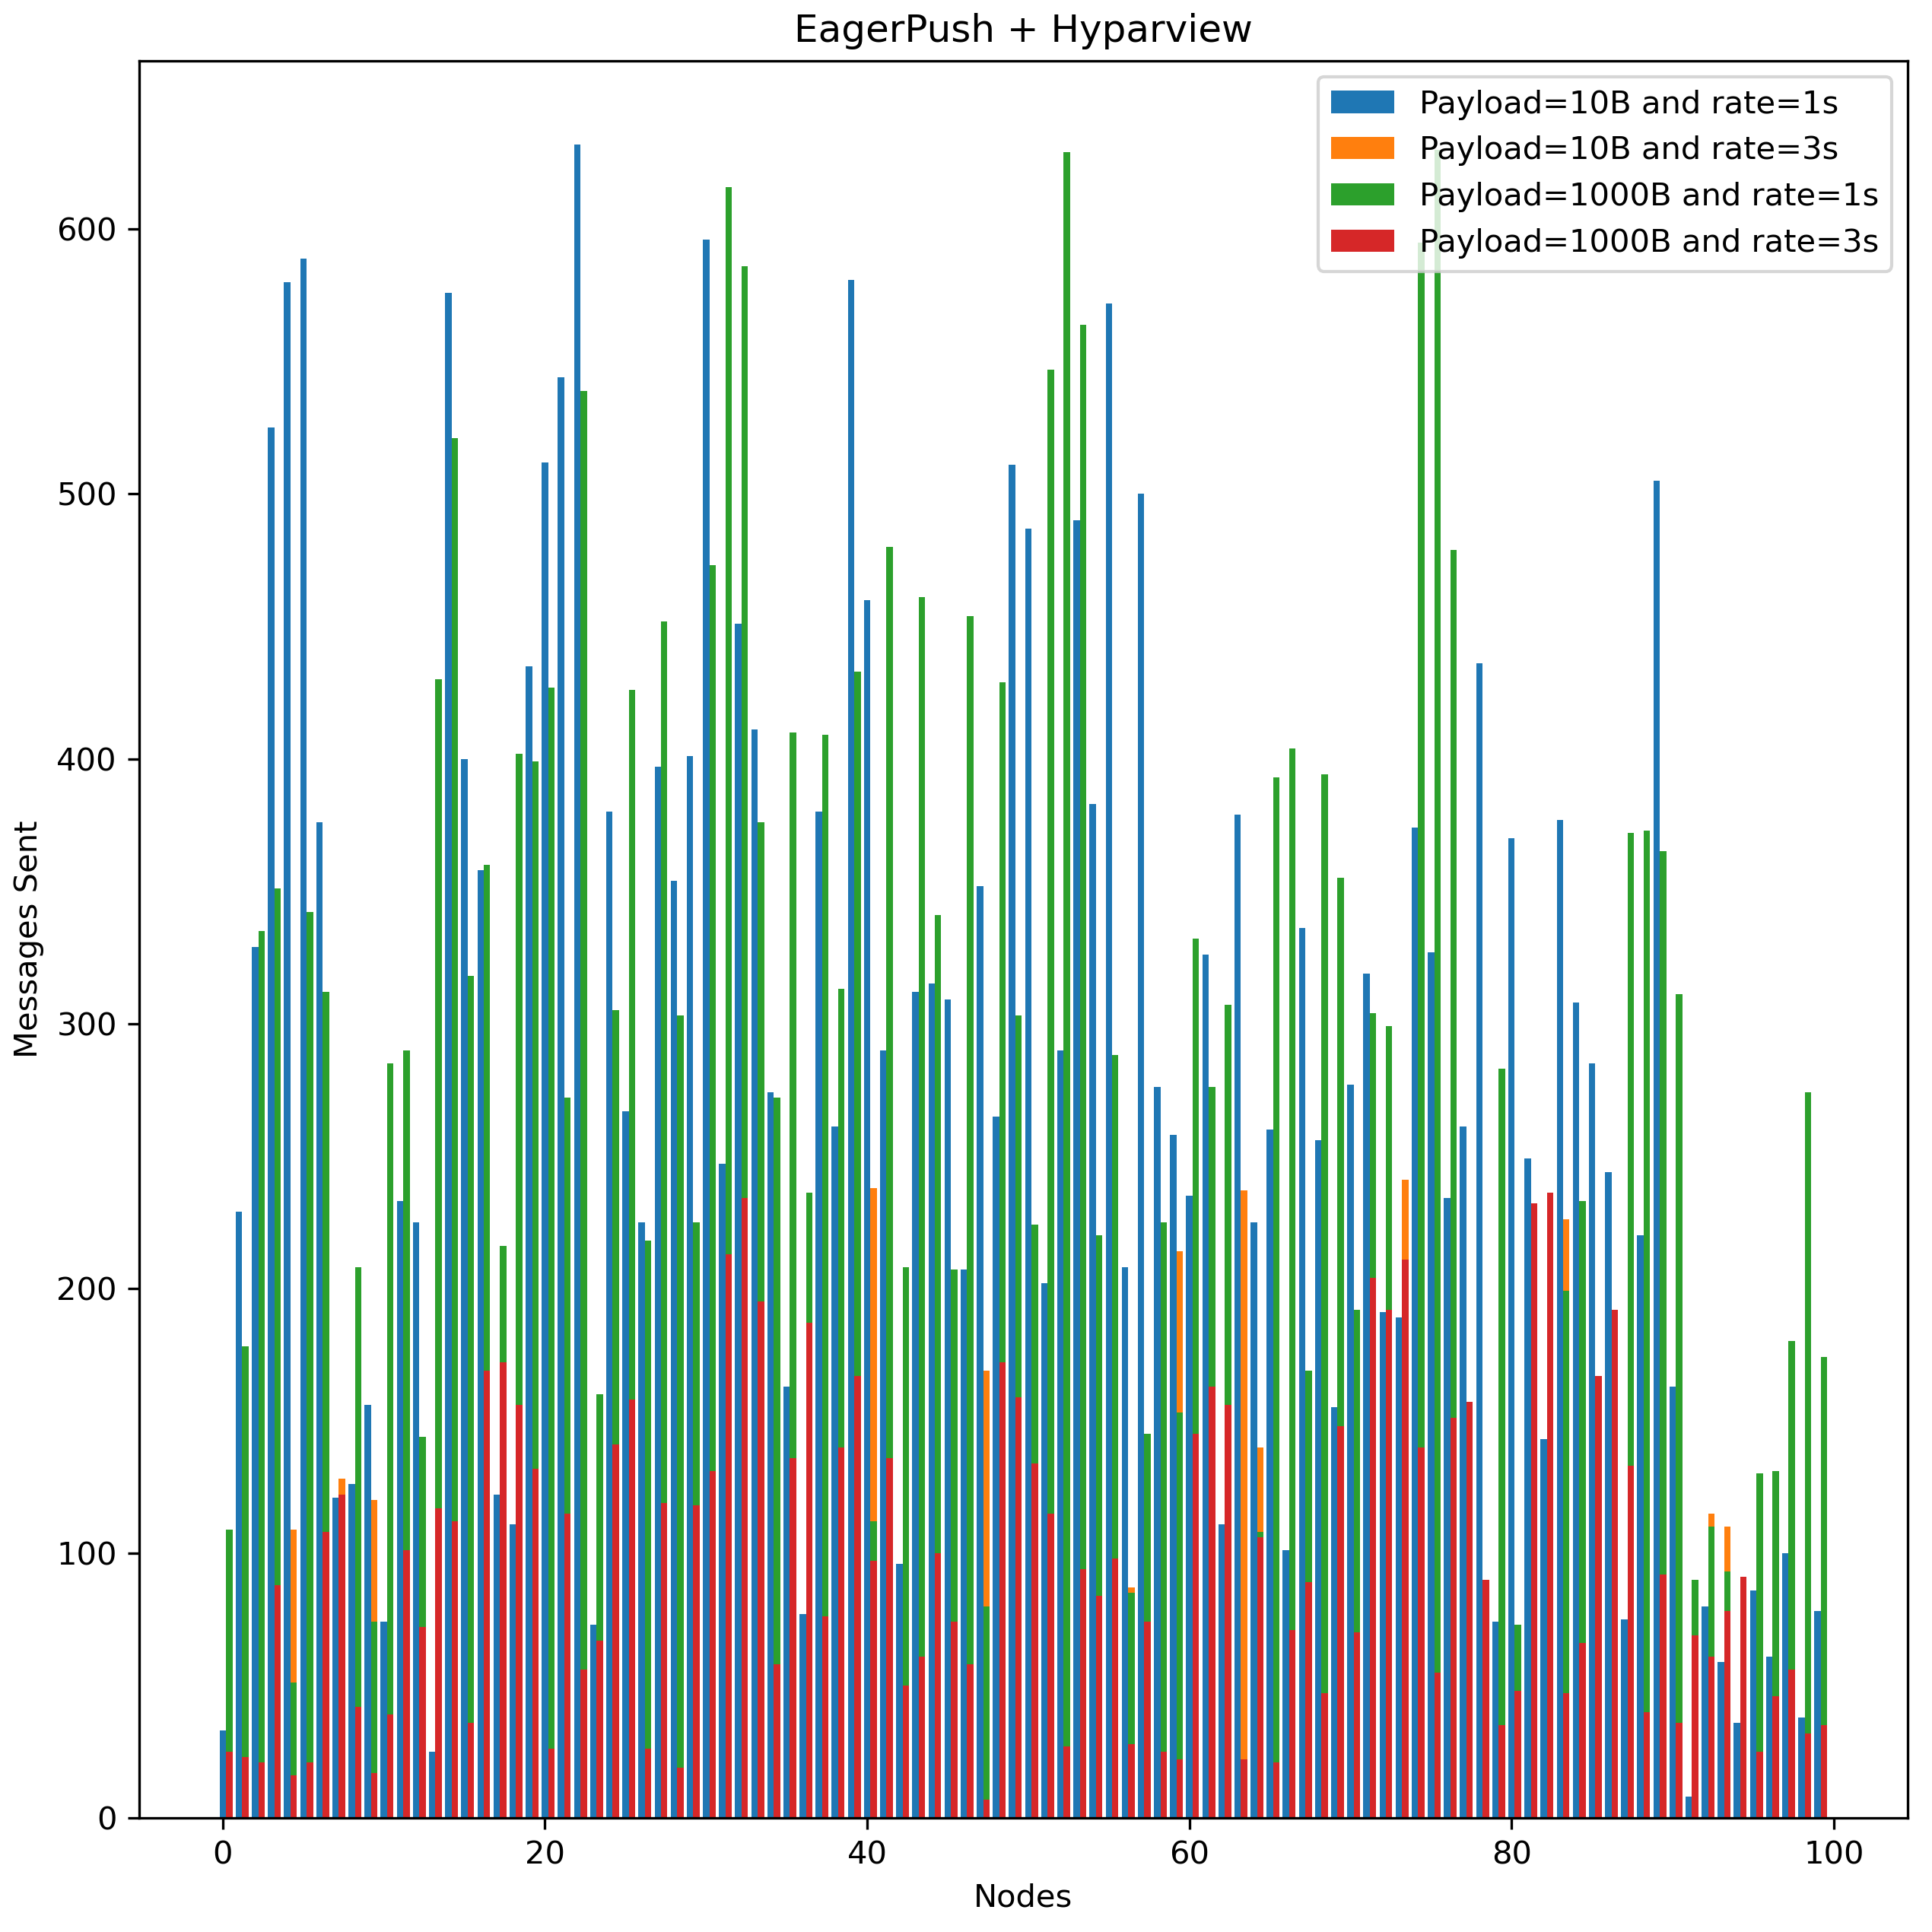
\includegraphics[width=0.4\textwidth]{images/EagerPush + HyparviewSent.png}
  \caption{EagerPush + Hyparview (Sent Messages)}
\end{figure}

\begin{figure}
  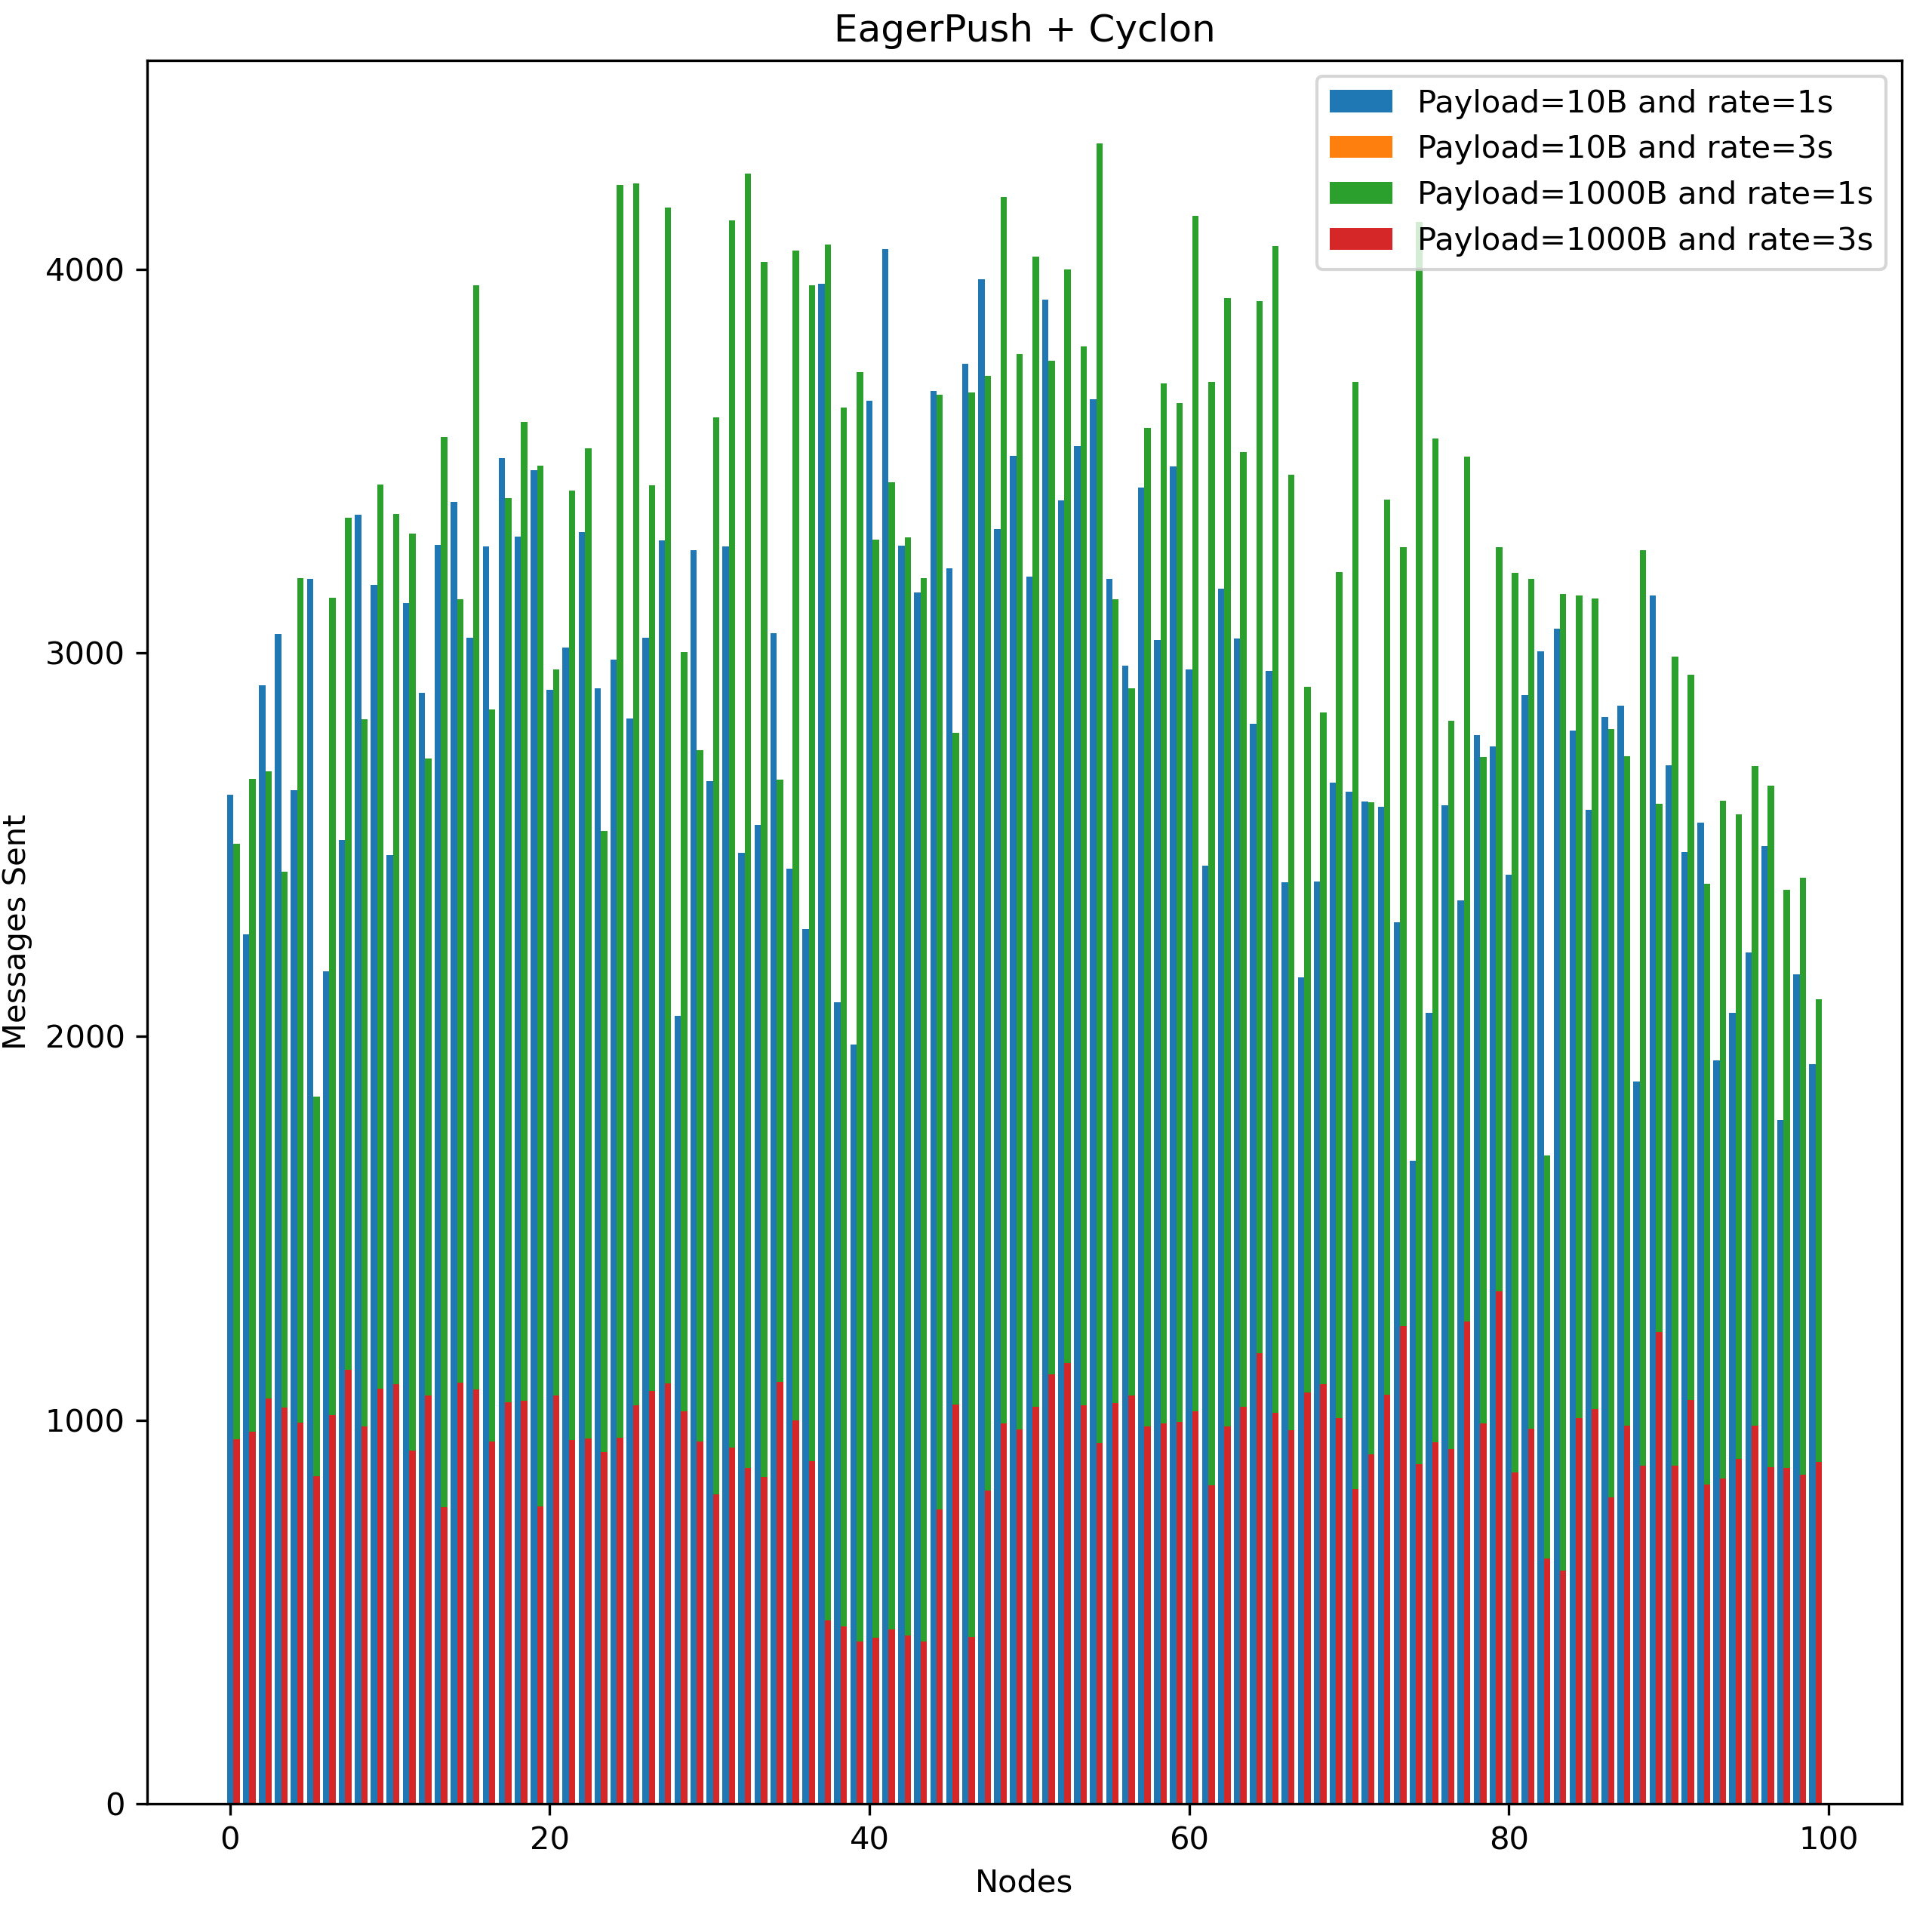
\includegraphics[width=0.4\textwidth]{images/EagerPush + CyclonSent.png}
  \caption{EagerPush + Cyclon (Sent Messages)}
\end{figure}

\begin{figure}
  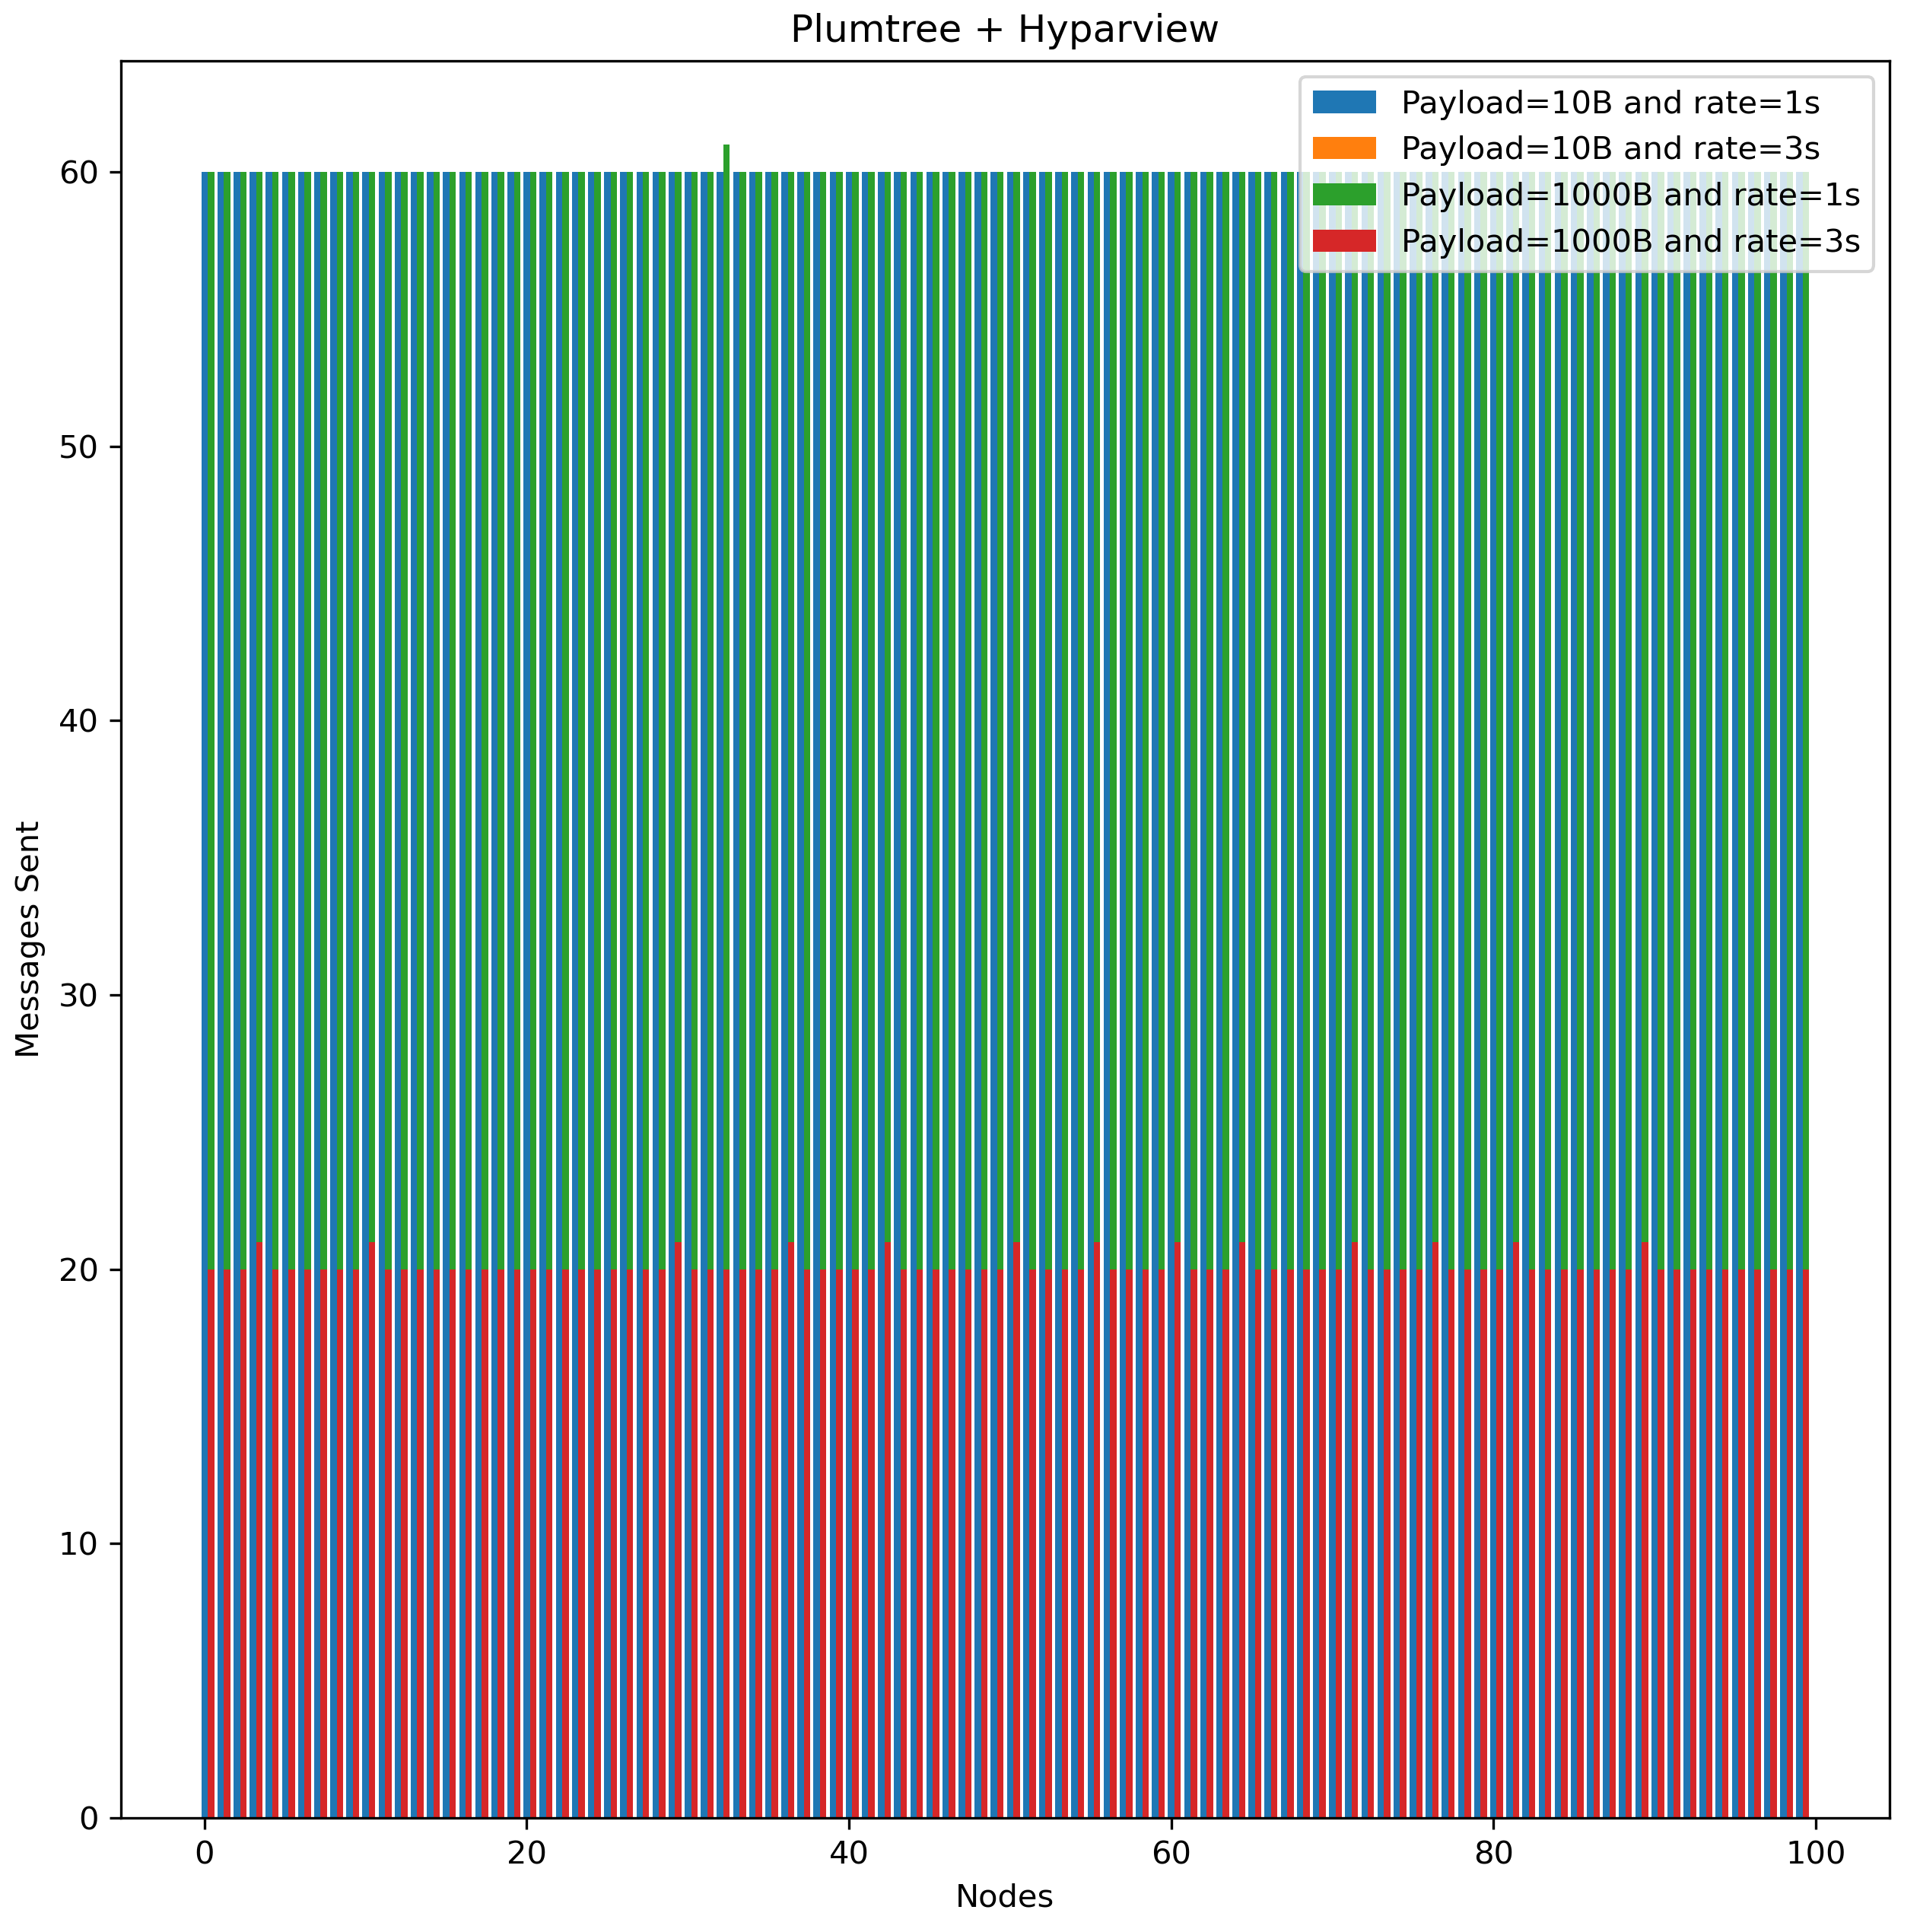
\includegraphics[width=0.4\textwidth]{images/Plumtree + HyparviewSent.png}
  \caption{Plumtree + Hyparview (Sent Messages)}
\end{figure}

\begin{figure}
  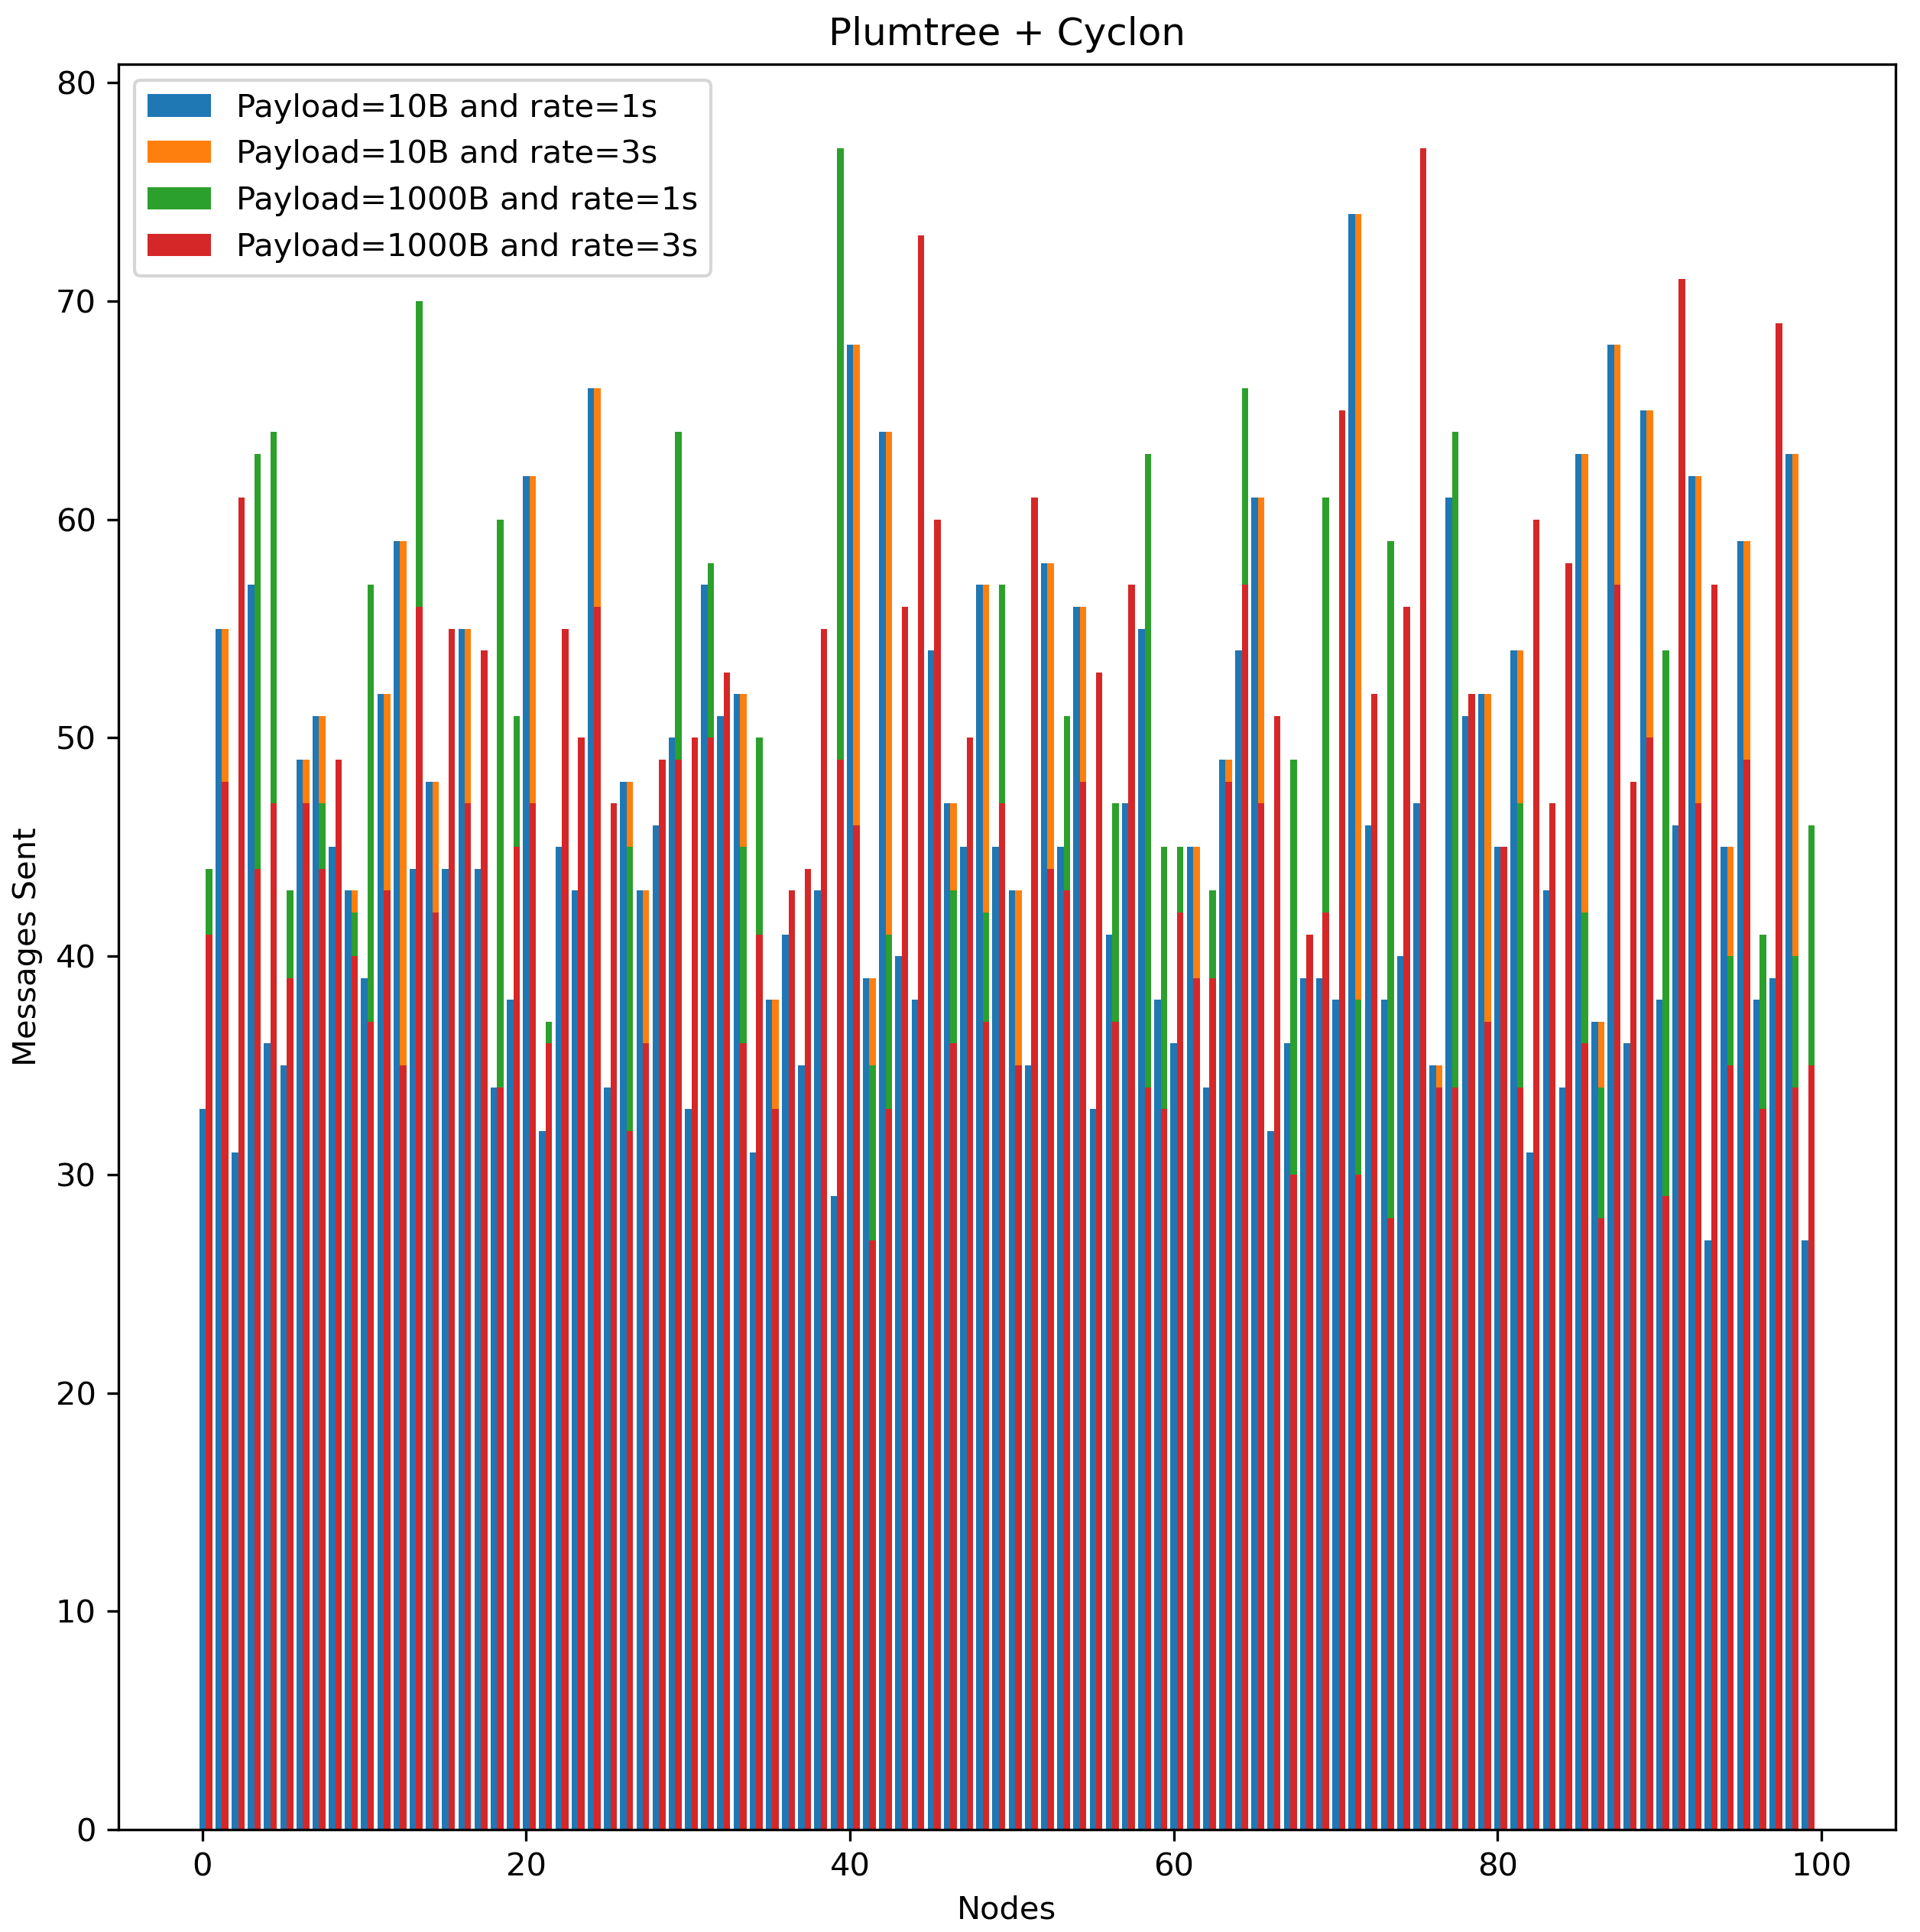
\includegraphics[width=0.4\textwidth]{images/Plumtree + CyclonSent.png}
  \caption{Plumtree + Cyclon (Sent Messages)}
\end{figure}

%--------------------------------------

\subsubsection{Failed Messages}

%TODO: Falar dos resultados
Nas \textit{Failed Messages}, houve um pequeno erro na geração dos gráficos, onde por lapso, no eixo vertical, os valores não estão ordenados. Porém dá para ter uma percepção geral dos resultados, principalmente nos gráficos onde o algoritmo de \textit{membership} utilizado foi o HyParView, onde se nota claramente que 90\% das barradas, independentemente das configurações utilizadas, estão com 0 mensagens falhadas. No entanto utilizando o Cyclon já se verifica uma maior discrepância nos resultados.

\begin{figure}
  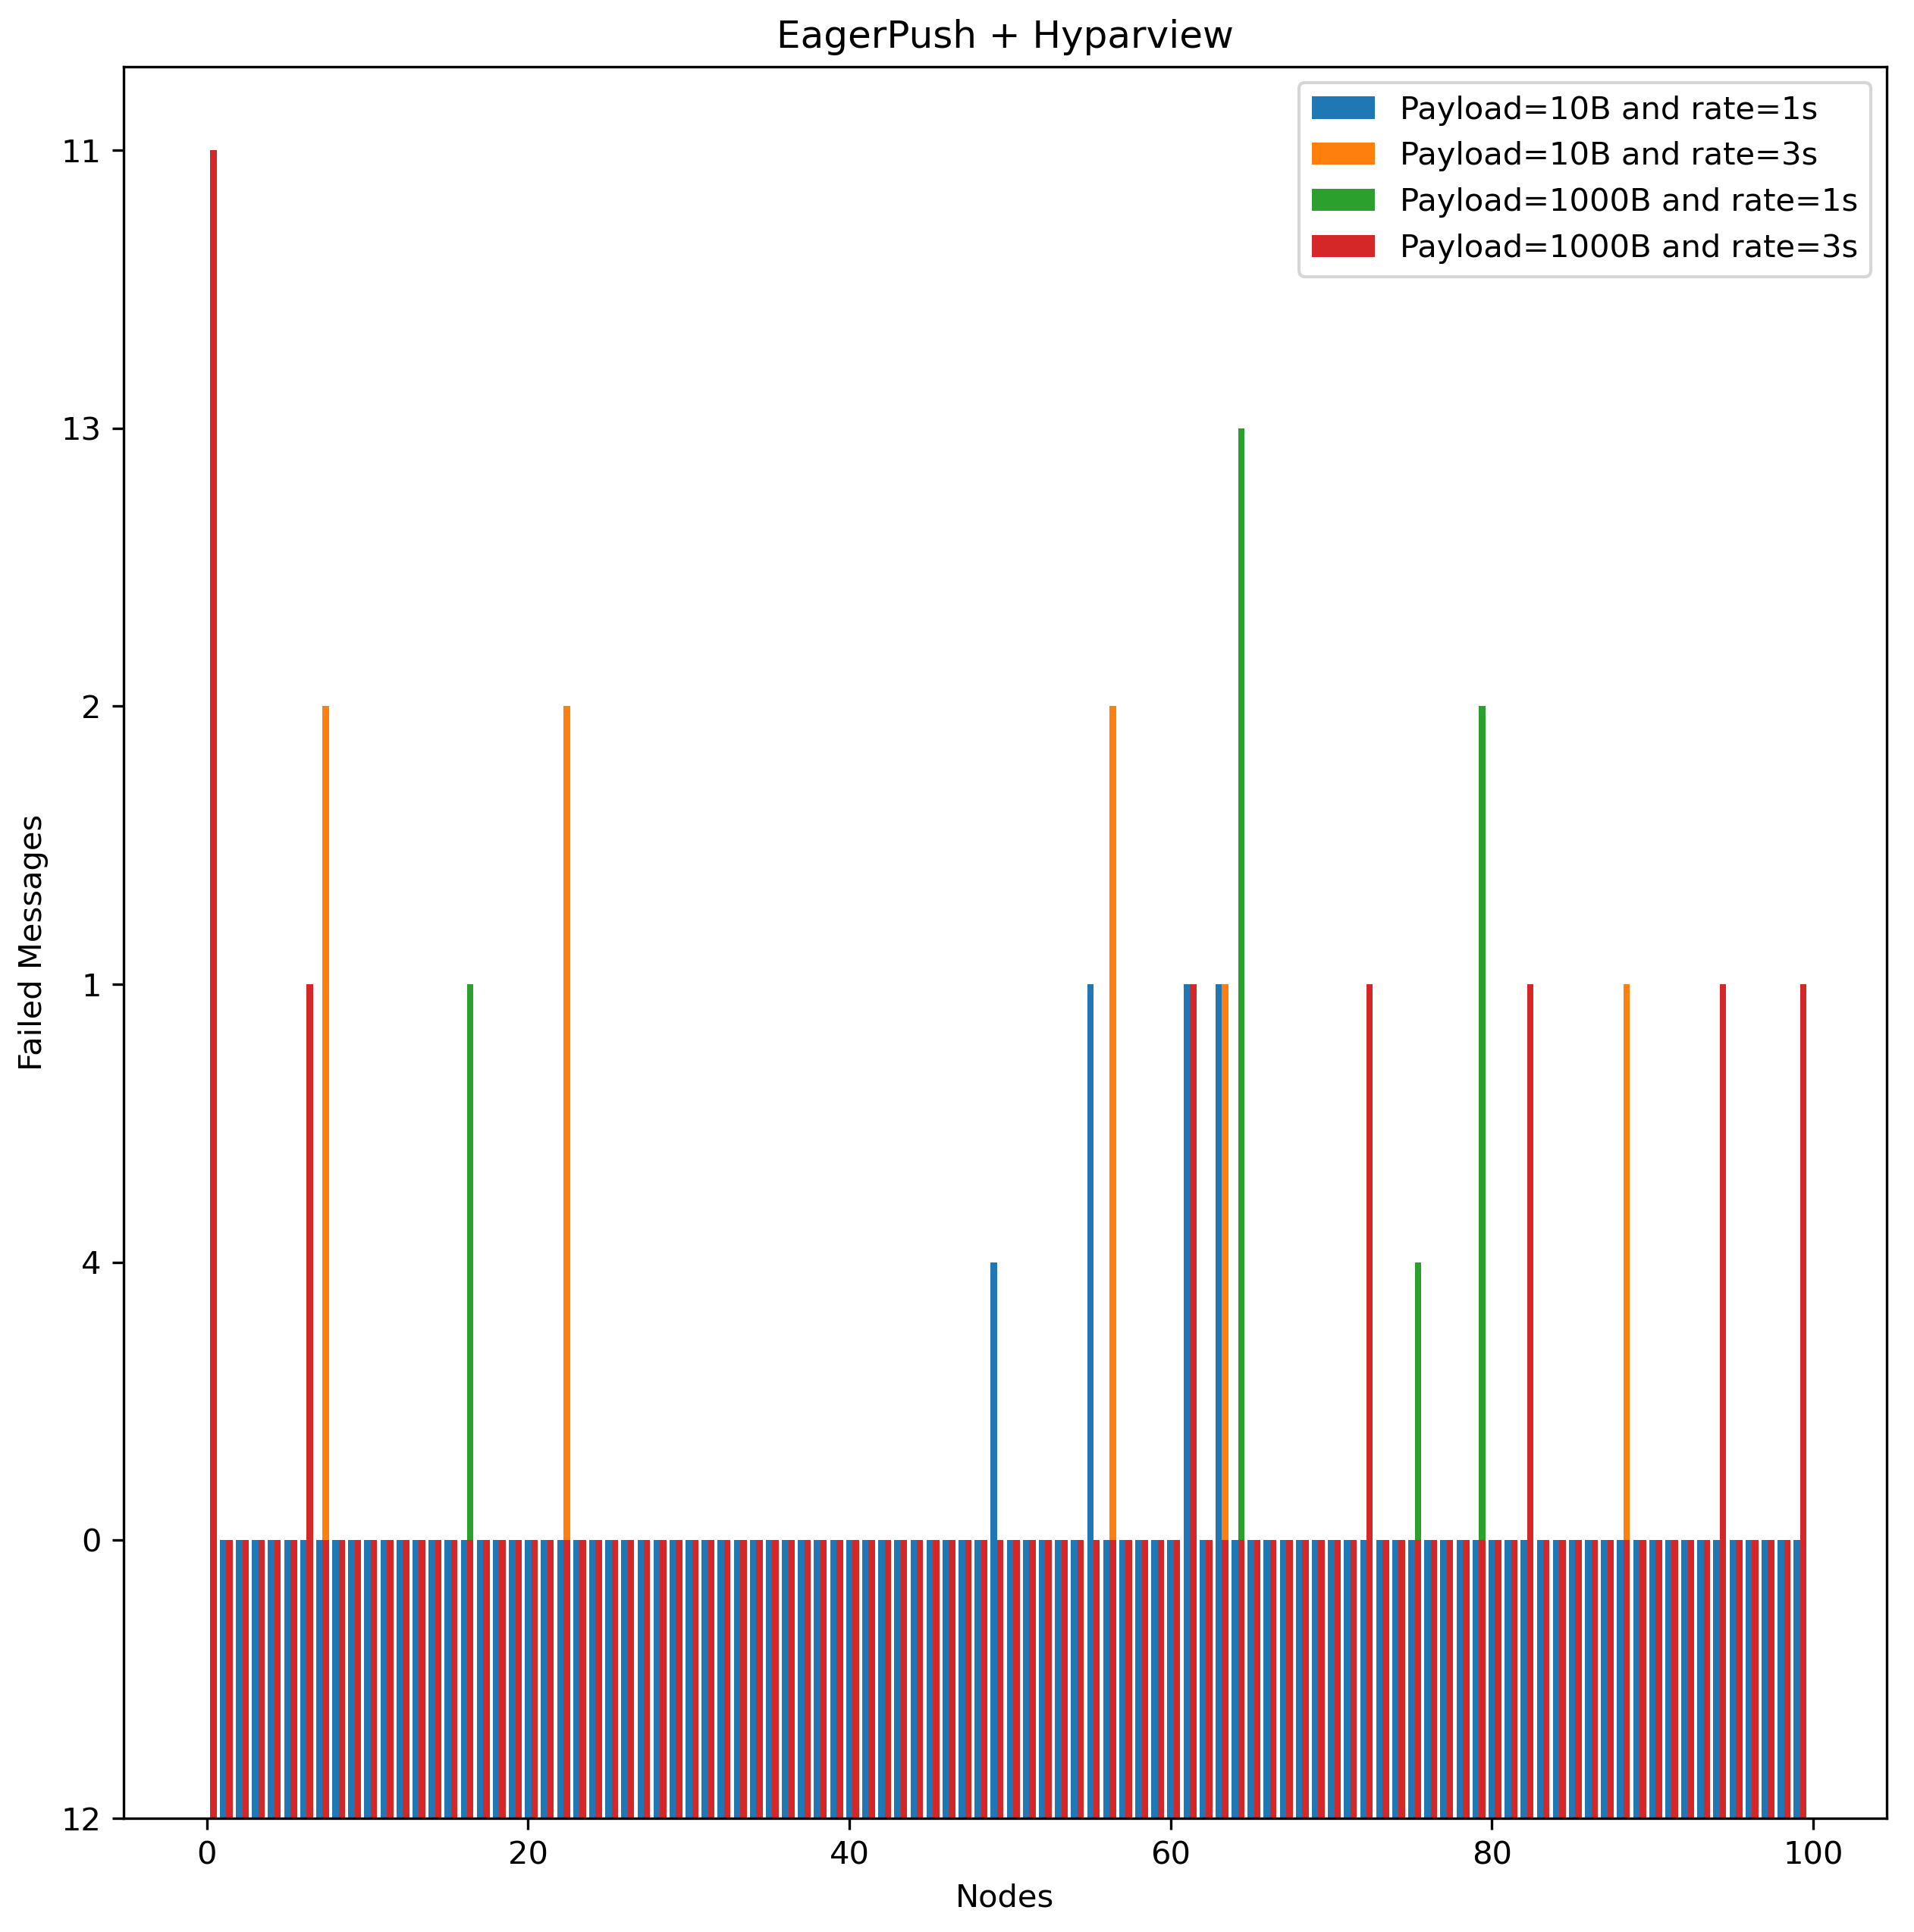
\includegraphics[width=0.4\textwidth]{images/EagerPush + HyparviewFailedMessages.png}
  \caption{EagerPush + Hyparview (Failed Messages)}
\end{figure}

\begin{figure}
  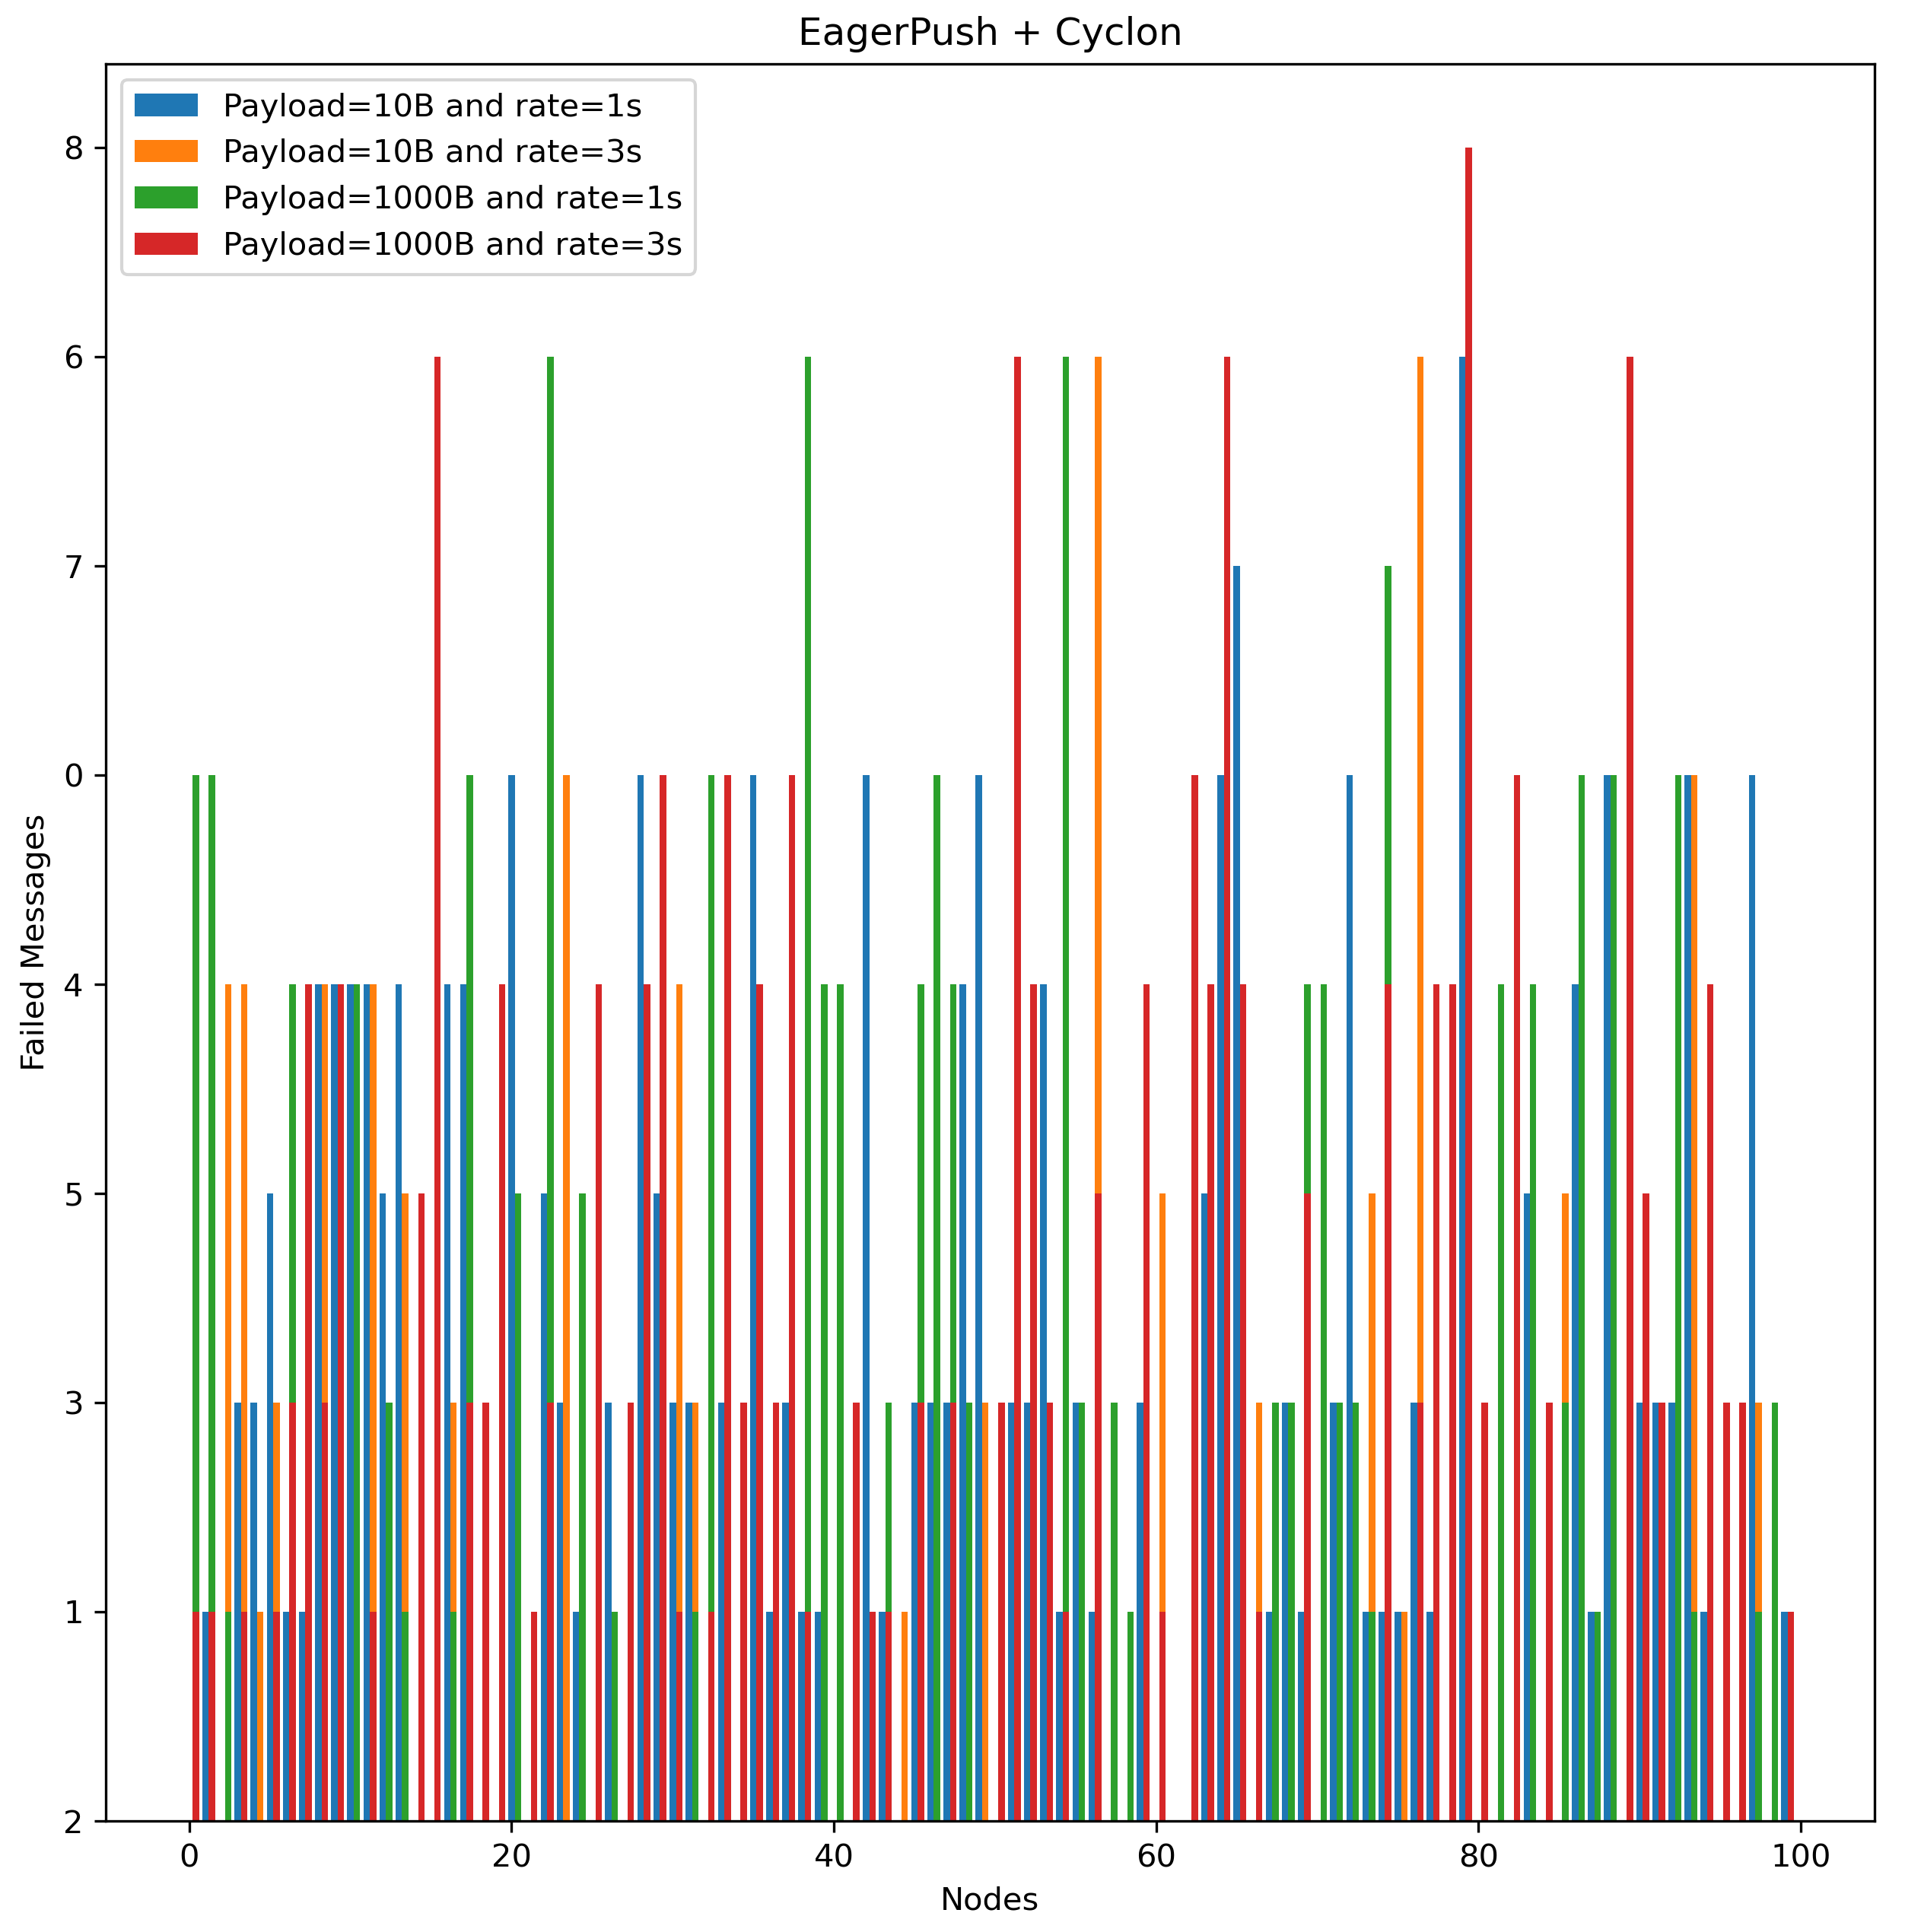
\includegraphics[width=0.4\textwidth]{images/EagerPush + CyclonFailedMessages.png}
  \caption{EagerPush + Cyclon (Failed Messages)}
\end{figure}

\begin{figure}
  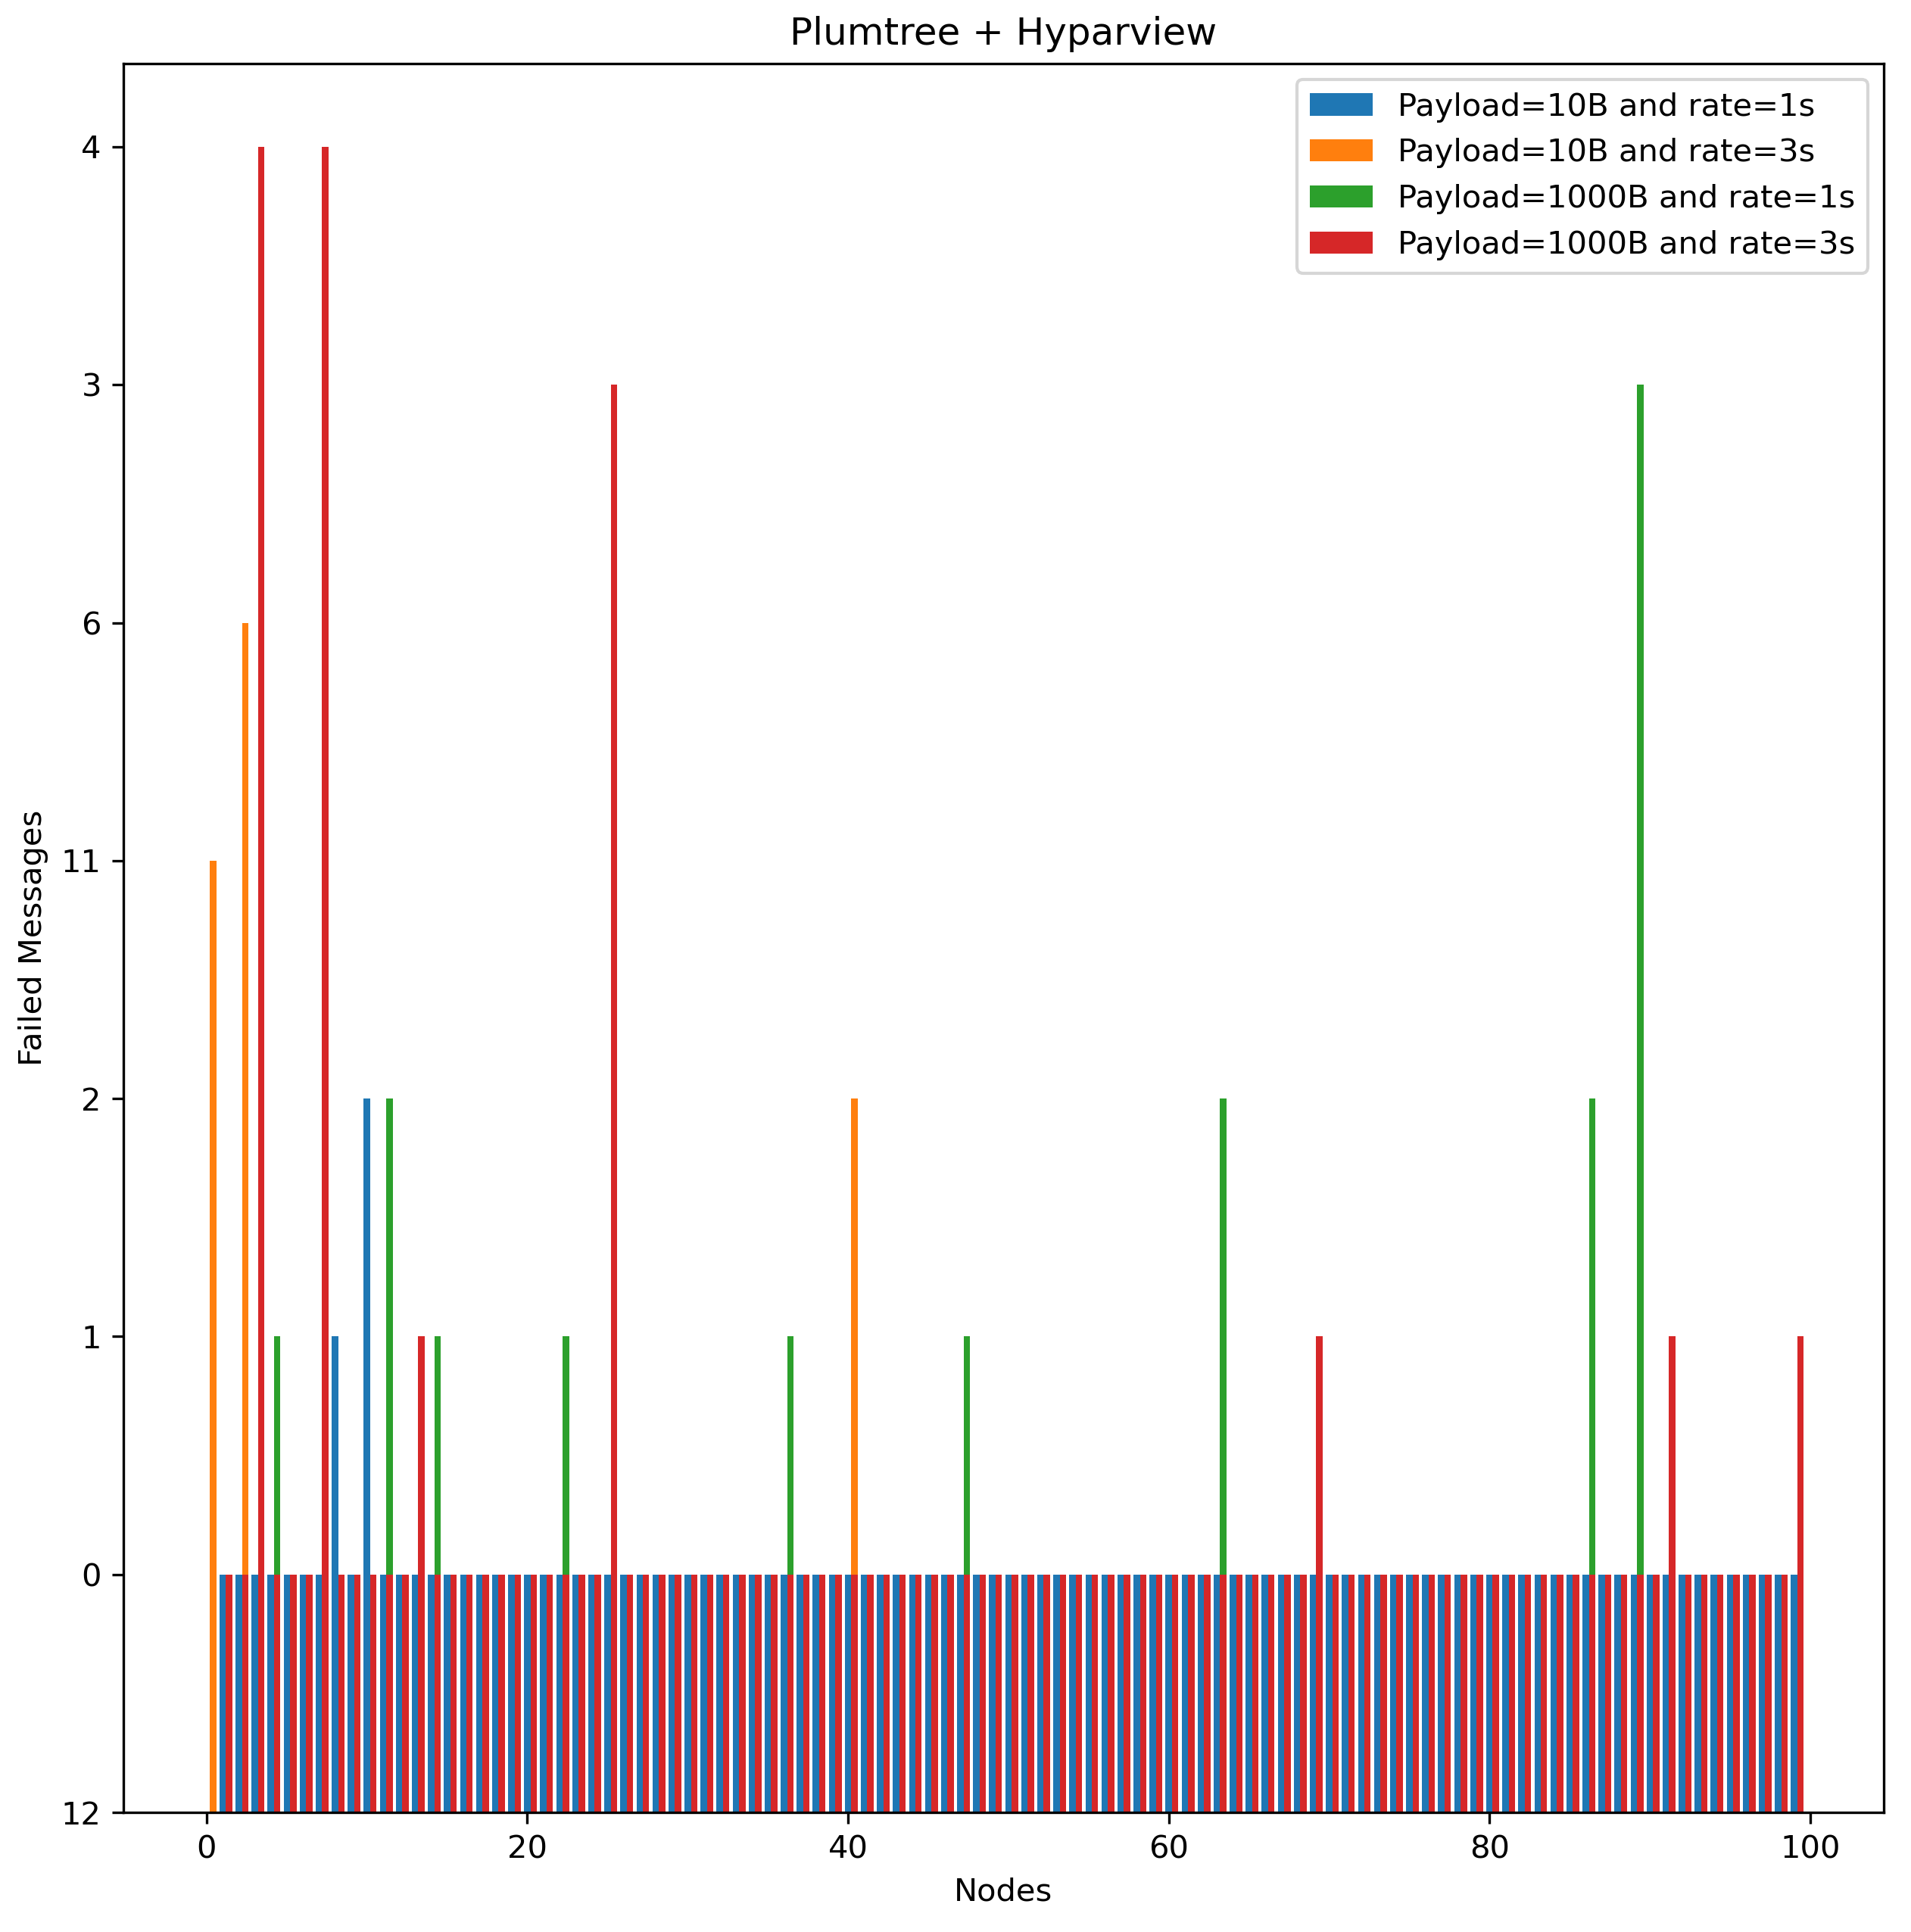
\includegraphics[width=0.4\textwidth]{images/Plumtree + HyparviewFailedMessages.png}
  \caption{Plumtree + Hyparview (Failed Messages)}
\end{figure}

\begin{figure}
  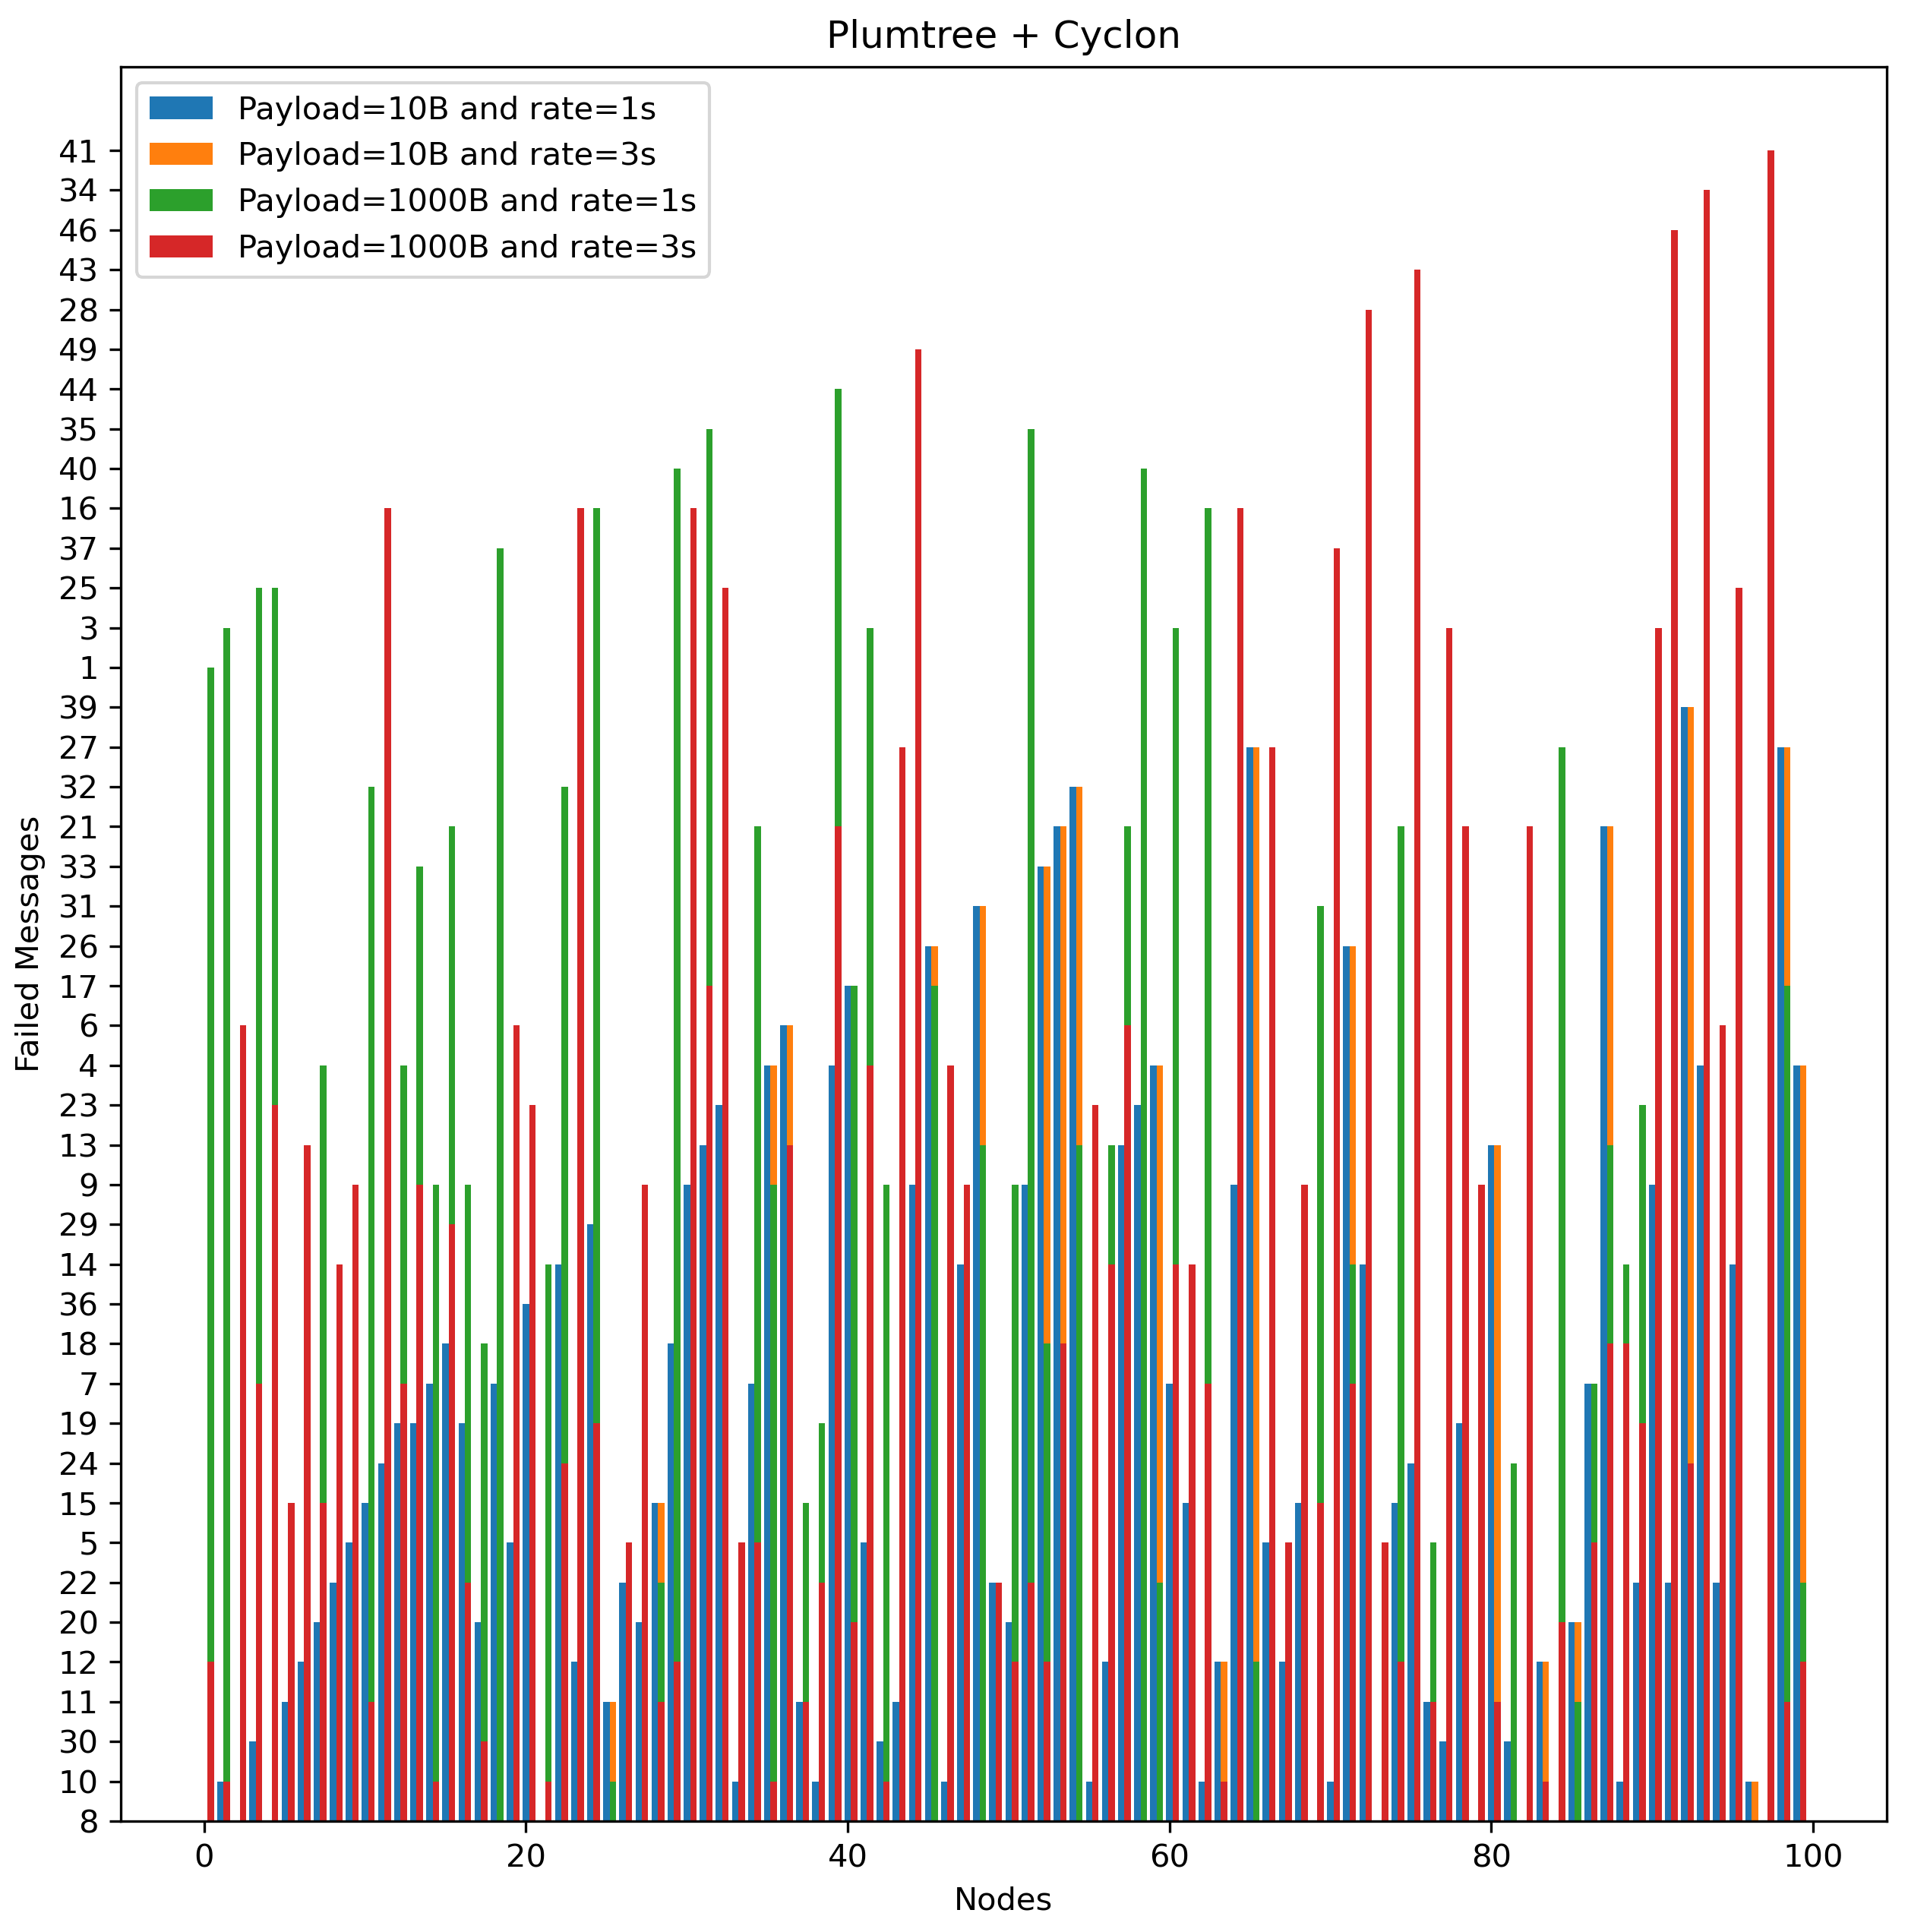
\includegraphics[width=0.4\textwidth]{images/Plumtree + CyclonFailedMessages.png}
  \caption{Plumtree + Cyclon (Failed Messages)}
\end{figure}

%--------------------------------------

\subsubsection{Latency} 
A latência media do algoritmo de \textit{broadcast} foi calculada da seguinte maneira: A partir do momento em que uma mensagem é enviada pela primeira vez para a rede, até chegar finalmente ao último processo que a recebeu. 
Como dito anteriormente, é possível verificar que houve problemas a medir a latência quando o algoritmo usado no teste era o Plumtree.
%TODO: Falar dos resultados

\paragraph{}

\begin{tabular}{ |p{3cm}||p{0.68cm}|p{0.69 cm}|p{0.67cm}|p{0.67cm}|}
\hline
 Parameters / Algotithm &E + H&E + C&P + H &P + C\\
\hline
\hline
Payload=10B, BR=1s & 9.12s & 61.27s & 0.0s & 0.0s\\
\hline
Payload=10B, BR=3s & 5.06s & 23.52s & 0.0s & 0.0s\\
\hline
Payload=10MB, BR=1s & 10.26s& 112.67s & 0.0s & 0.0s\\
\hline
Payload=10MB, BR=3s& 3.74s & 25.75s & 0.0s& 0.0s\\
\hline
\end{tabular}

%--------------------------------------
%--------------------------------------
%--------------------------------------

\subsection{Discussion}
%-->discussão dos resultados um a um
%-Explicar o que esta no gráfico
%-Extrair conclusões
%Juntar gráficos e cores dos gráficos

%TODO:Compração entre algoritmos

De acordo com os dados apresentados nos gráficos, é possível verificar que no gráfico da figura 7 (Plumtree + HyParView), que o total de mensagens enviadas pelos nós correspondem ao esperado. Independentemente do tamanho do \textit{payload}, e sabendo que cada nó esteve a executar durante 60 segundos, o esperado utilizando uma taxa de transmissão de 1 e 3 segundos, deu o resultado respectivo de 60 e 20 como esperado.
No entanto, nas outras combinações de algoritmos, verificou-se uma grande duplicação de mensagens não correspondendo ao valor esperado. Estes resultados podem ser devidos a vários factores, tais como \textit{bugs} na implementação dos algoritmos ou no processamento dos \textit{logs}.

Relativamente ao teste da totalidade de mensagens falhadas é possível verificar que usando as combinações com o HyParView a taxa de mensagens falhadas é pouco representativa, porem na combinação  Plumtree + Cyclon é possível verificar que houve um grande número de mensagens falhadas. No  Eager Push + Cyclon apesar de se verificar algum numero de mensagens falhadas, a sua percentagem relativamente ao total de mensagens enviadas ( 60 para um\textit{ rate} de 1s e 20 para um rate de 3s) é inferior.

No caso da\textit{ reliability}, é possível verificar que para todas as combinações de algoritmos excepto o Plumtree + Cyclon, os resultados foram bastante positivos, tendo apenas uma fracção muito pequena de nós onde a reliability foi inferior ao esperado. No caso do Plumtree + Cyclon é possível verificar uma instabilidade na maioria dos nós da rede possivelmente devido a problemas de implementação, ou possivelmente até mesmo devido a algumas instabilidades na rede do \textit{cluster}.

Por último, relativamente à latência é possível verificar que o HyParView relativamente ao Cyclon demonstra uma menor latência independentemente das configurações. Mais não podemos concluir devido aos dados estatísticos do Plumtree, que em todos os testes deu uma media de 0.0s, o que impossibilitou uma comparação mais pormenorizada para com as outras combinações de algoritmos.